\chapter{Elastic Load Balancing (ELB)}\label{ch:elastic-load-balancing}

Elastic Load Balancing is used to automatically scale your EC2 instances to meet any changes in demand from your users.
ELB can be used to both scale up or down the instance's resources to ensure that your application is kept performant and
available regardless of how many users visit.
It is also possible to scale down the resources again, after the spike in usage has passed, to save money when it comes
to billing and ensure you aren't paying for any additional resources that are not being used.

1. Creation of new AMI

\begin{itemize}
    \item Selection of AMI previously created and then "Create Instance from AMI" option (elb/elb-instance-from-ami)
    \item AMI selected to use same instance as "Group4-EC2" so everything is the same (elb/elb-instance-2-name)
    \item Same keypair used, so it is easier to switch between both instances (elb/elb-instance-2-type-and-keypair)
    Network Settings
    \item VPC set to be Group4 VPC  (created in Section~\ref{ch:vpc}) (elb/elb-instance-2-network-settings)
    \item Subnet set to be "Public Subnet 2" (elb/elb-instance-2-network-settings)
    \item Public IP auto-assigned (elb/elb-instance-2-network-settings)
    \item Existing security group of "Group4-Security-Group" selected to allow HTTP, HTTPS, SSH and MySQL traffic on the
    instance (elb/elb-instance-2-network-settings)
    \item Storage remains the same as previous instance (elb/elb-instance-2-storage-config)
    \item Second instance now created (elb/elb-instance-2-created)
\end{itemize}

2. Creation of target group

Now that there is 2 instances, they both need to be stored within a target group.

\begin{itemize}
    \item The Target Group type of "Instances" is selected - this will store both running instances of Digital-Ink in a group
    to be handled by the Load Balancer (elb/elb-target-group-basic-config)
    \item Target Group name of "Group4-Target-Group" given (elb/elb-target-group-basic-config)
    \item Protocol of HTTP and port 80 given (elb/elb-target-group-basic-config)
    \item Group4-VPC selected (elb/elb-vpc)
    \item The next screen asks for instances that will be registered to the Target Group to be selected
    \item The 2 running instances of Digital Ink are shown and added as targets through the "Include as pending below"
    button (elb/elb-register-targets)
    \item Target group now created, and contains both EC2 instances within them (elb/elb-target-group-created)
\end{itemize}

3. Creation of Load Balancer

\begin{itemize}
    \item The Target groups are not associated with a Load Balancer, so one will be created as an Application Load Balancer
    (elb/elb-load-balancer-created)
    \item Given the name of "Group4-Load-Balancer' (elb/elb-basic-config)
    \item Set to be internet facing and will handle ipv4 addresses (elb/elb-network-mapping)
    \item The security group of Group4-Security-Group is selected, which allows HTTP, HTTPS, SSH and MySQL traffic within
    the load balancer (elb/elb-security-groups-and-listeners)
    \item In the event that either of the web apps goes down, it will be forwarded to the Group4-Target-Group, which will then
    display the available instance (elb/elb-security-groups-and-listeners)
    \item Could not create Global Accelerator due to permissions issue (Future improvement) (elb/elb-accelerator)
    \item Summary (elb/elb-summary)
    \item Load balancer created (elb/elb-created)
    \item When the load balancer is visited at
    \href{http://http://group4-load-balancer-1914525647.us-east-1.elb.amazonaws.com/}{http://http://group4-load-balancer-1914525647.us-east-1.elb.amazonaws.com/},
    the website is shown (elb/elb-working)
\end{itemize}

\begin{figure}[!htbp]
    \centering
    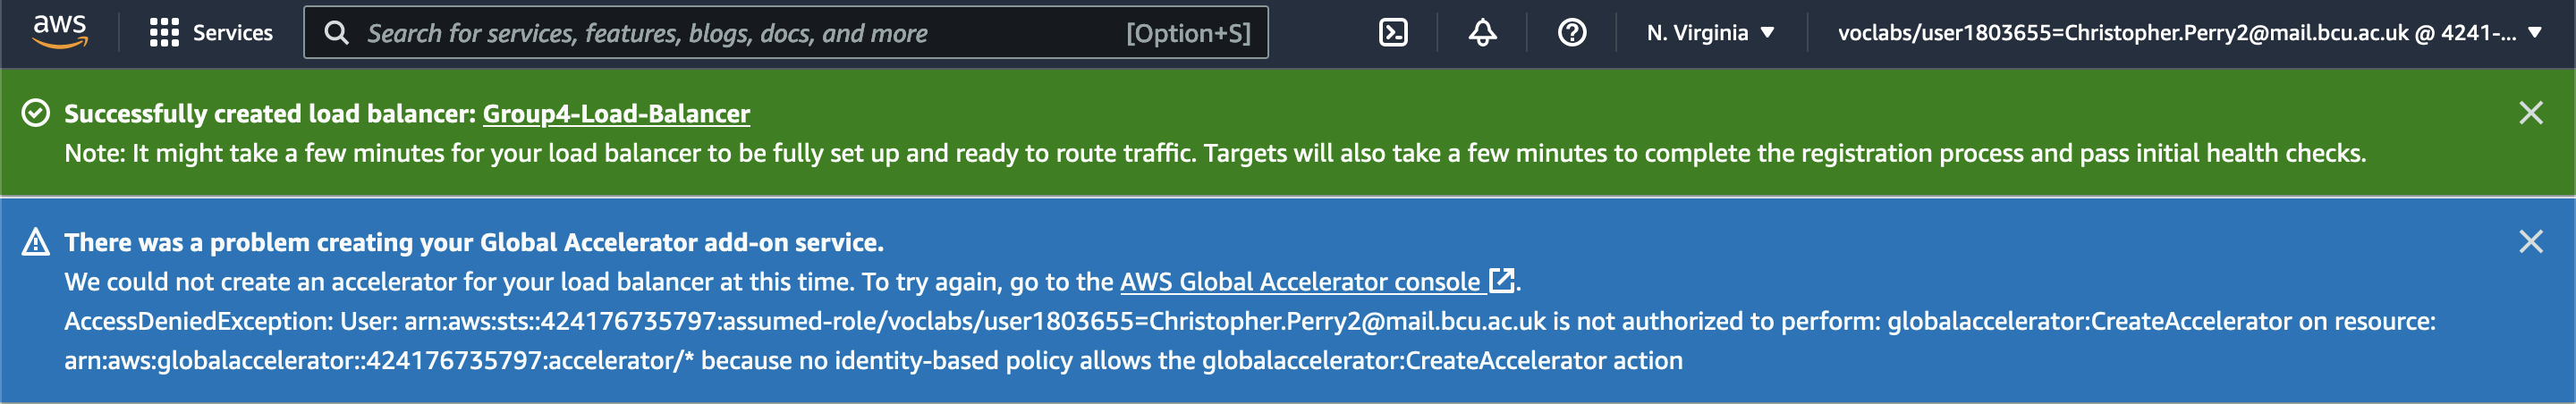
\includegraphics[width=\textwidth]{resources/elb/elb-accelerator.png}
    \caption{Elastic Load Balancing}
    \label{fig:elb-accelerator}
\end{figure}

\begin{figure}[!htbp]
    \centering
    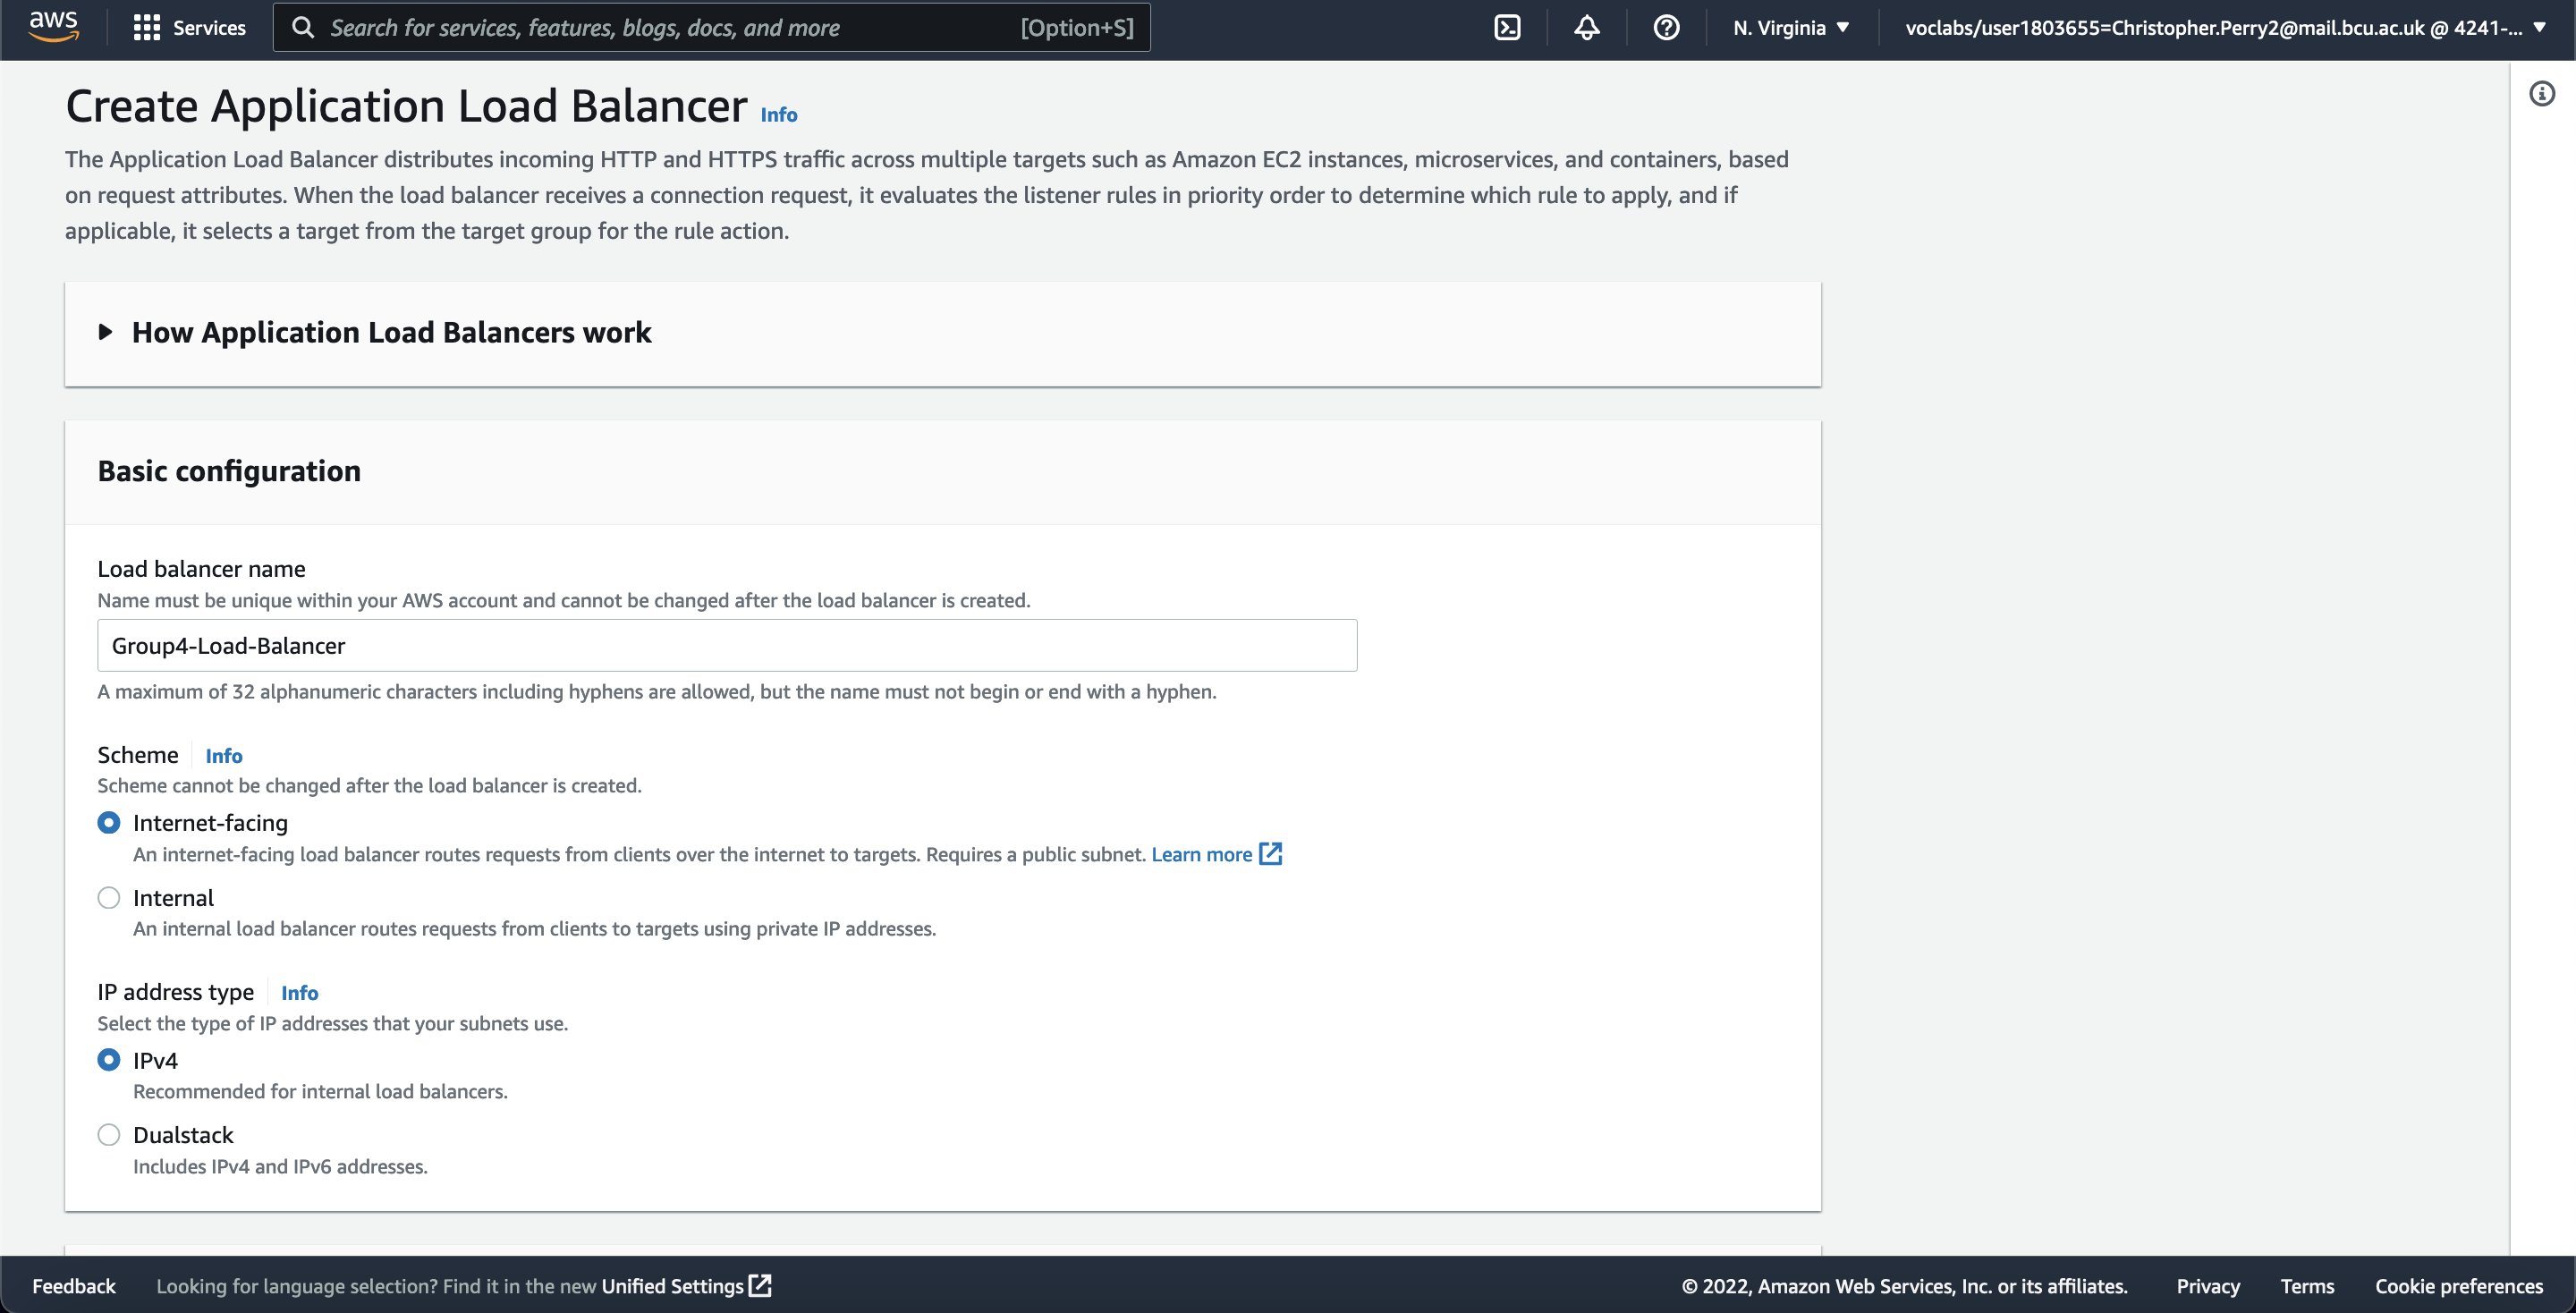
\includegraphics[width=\textwidth]{resources/elb/elb-basic-config.png}
    \caption{Elastic Load Balancing}
    \label{fig:elb-basic-config}
\end{figure}
\begin{figure}[!htbp]
    \centering
    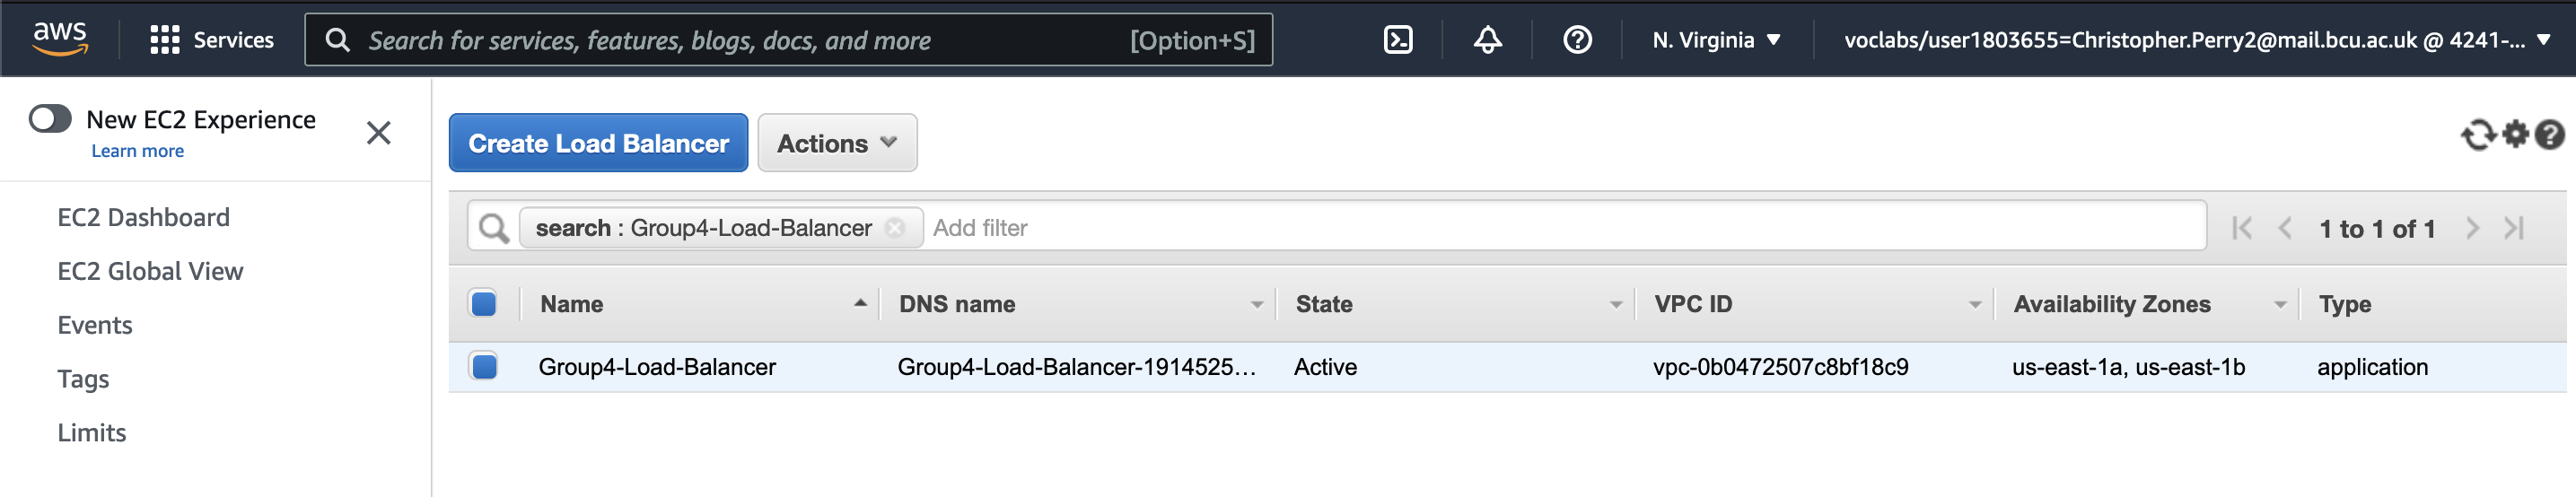
\includegraphics[width=\textwidth]{resources/elb/elb-created.png}
    \caption{Elastic Load Balancing}
    \label{fig:elb-created}
\end{figure}
\begin{figure}[!htbp]
    \centering
    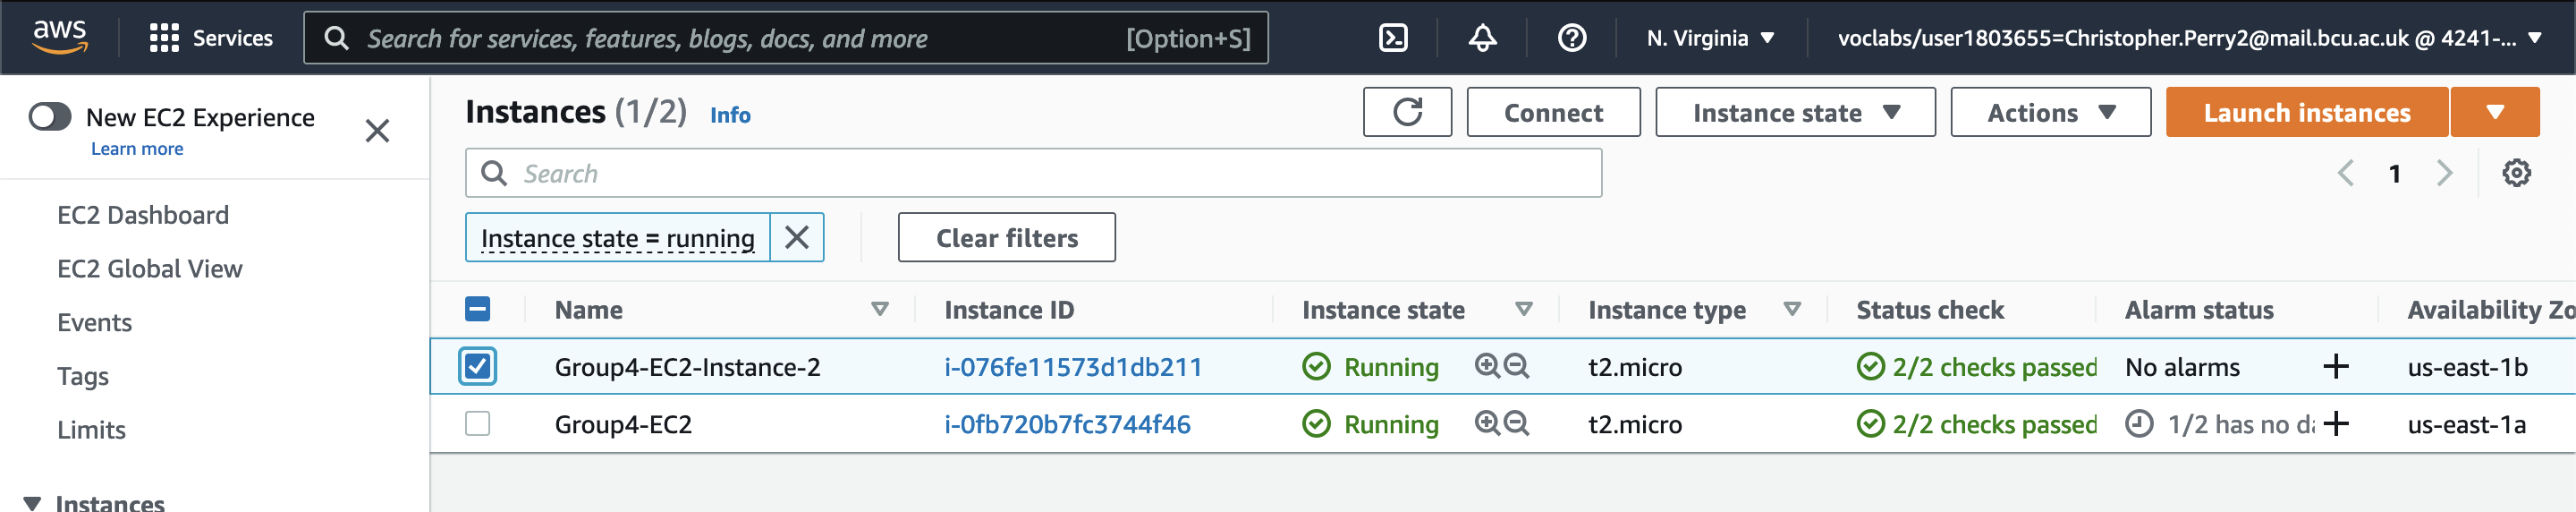
\includegraphics[width=\textwidth]{resources/elb/elb-instance-2-created.png}
    \caption{Elastic Load Balancing}
    \label{fig:elb-instance-2-create}
\end{figure}
\begin{figure}[!htbp]
    \centering
    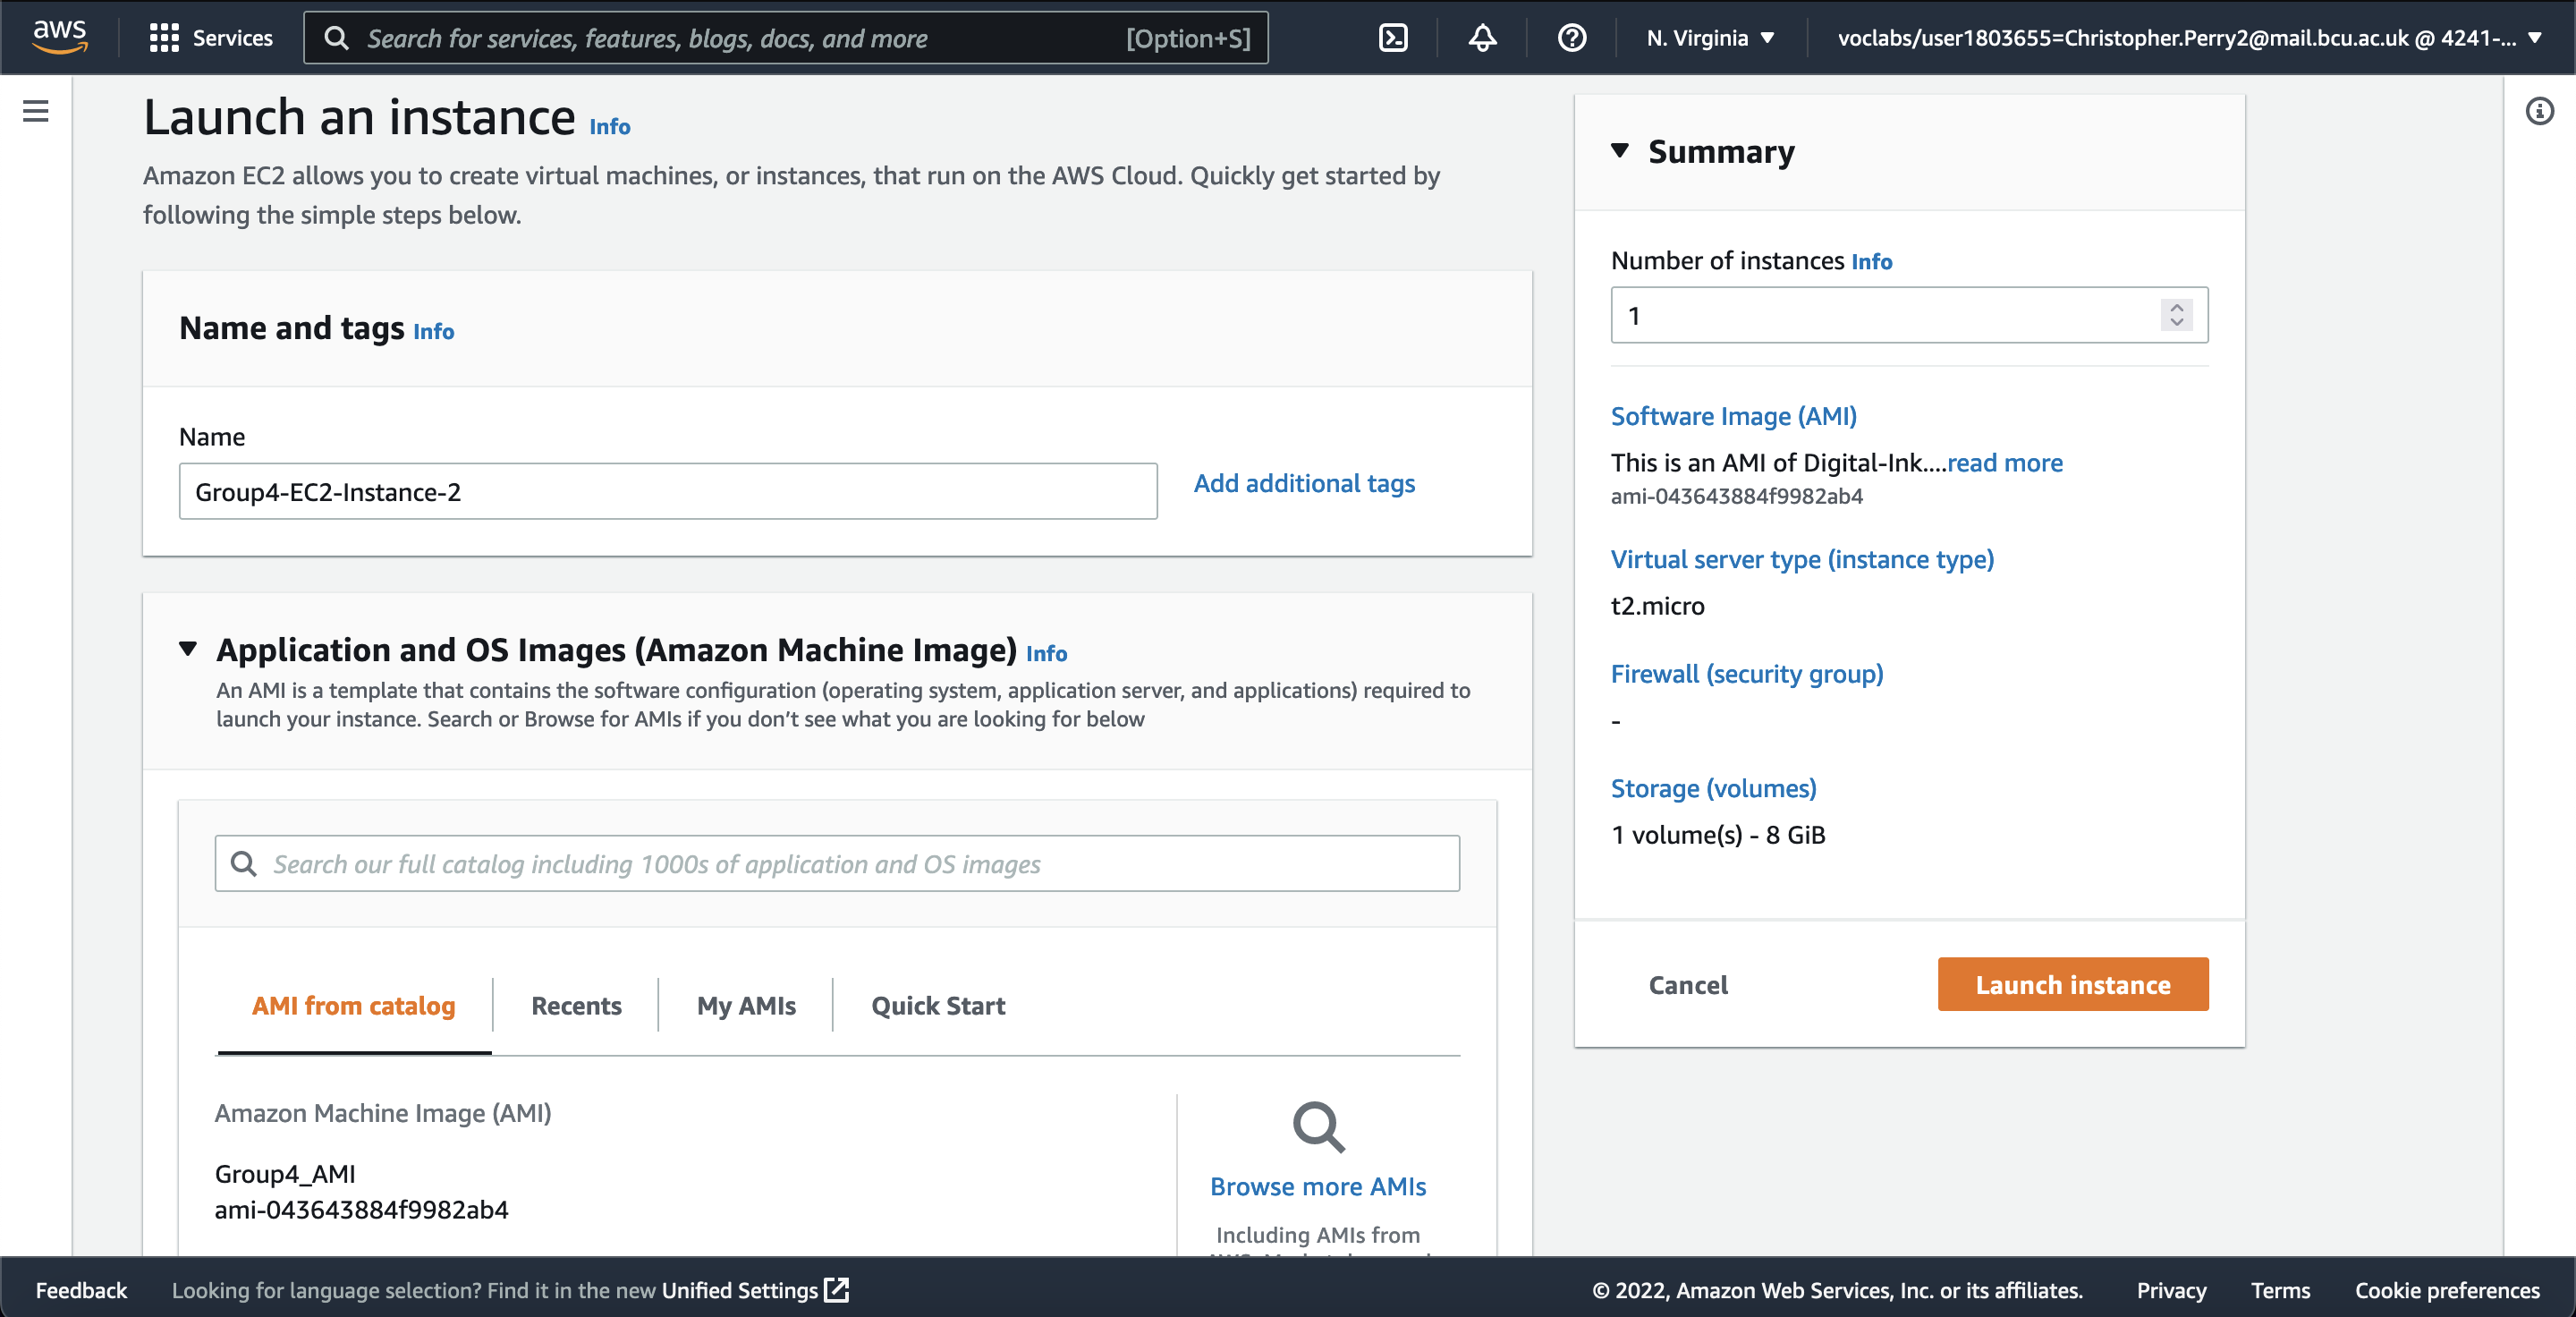
\includegraphics[width=\textwidth]{resources/elb/elb-instance-2-name.png}
    \caption{Elastic Load Balancing}
    \label{fig:elb-instance-2-name}
\end{figure}
\begin{figure}[!htbp]
    \centering
    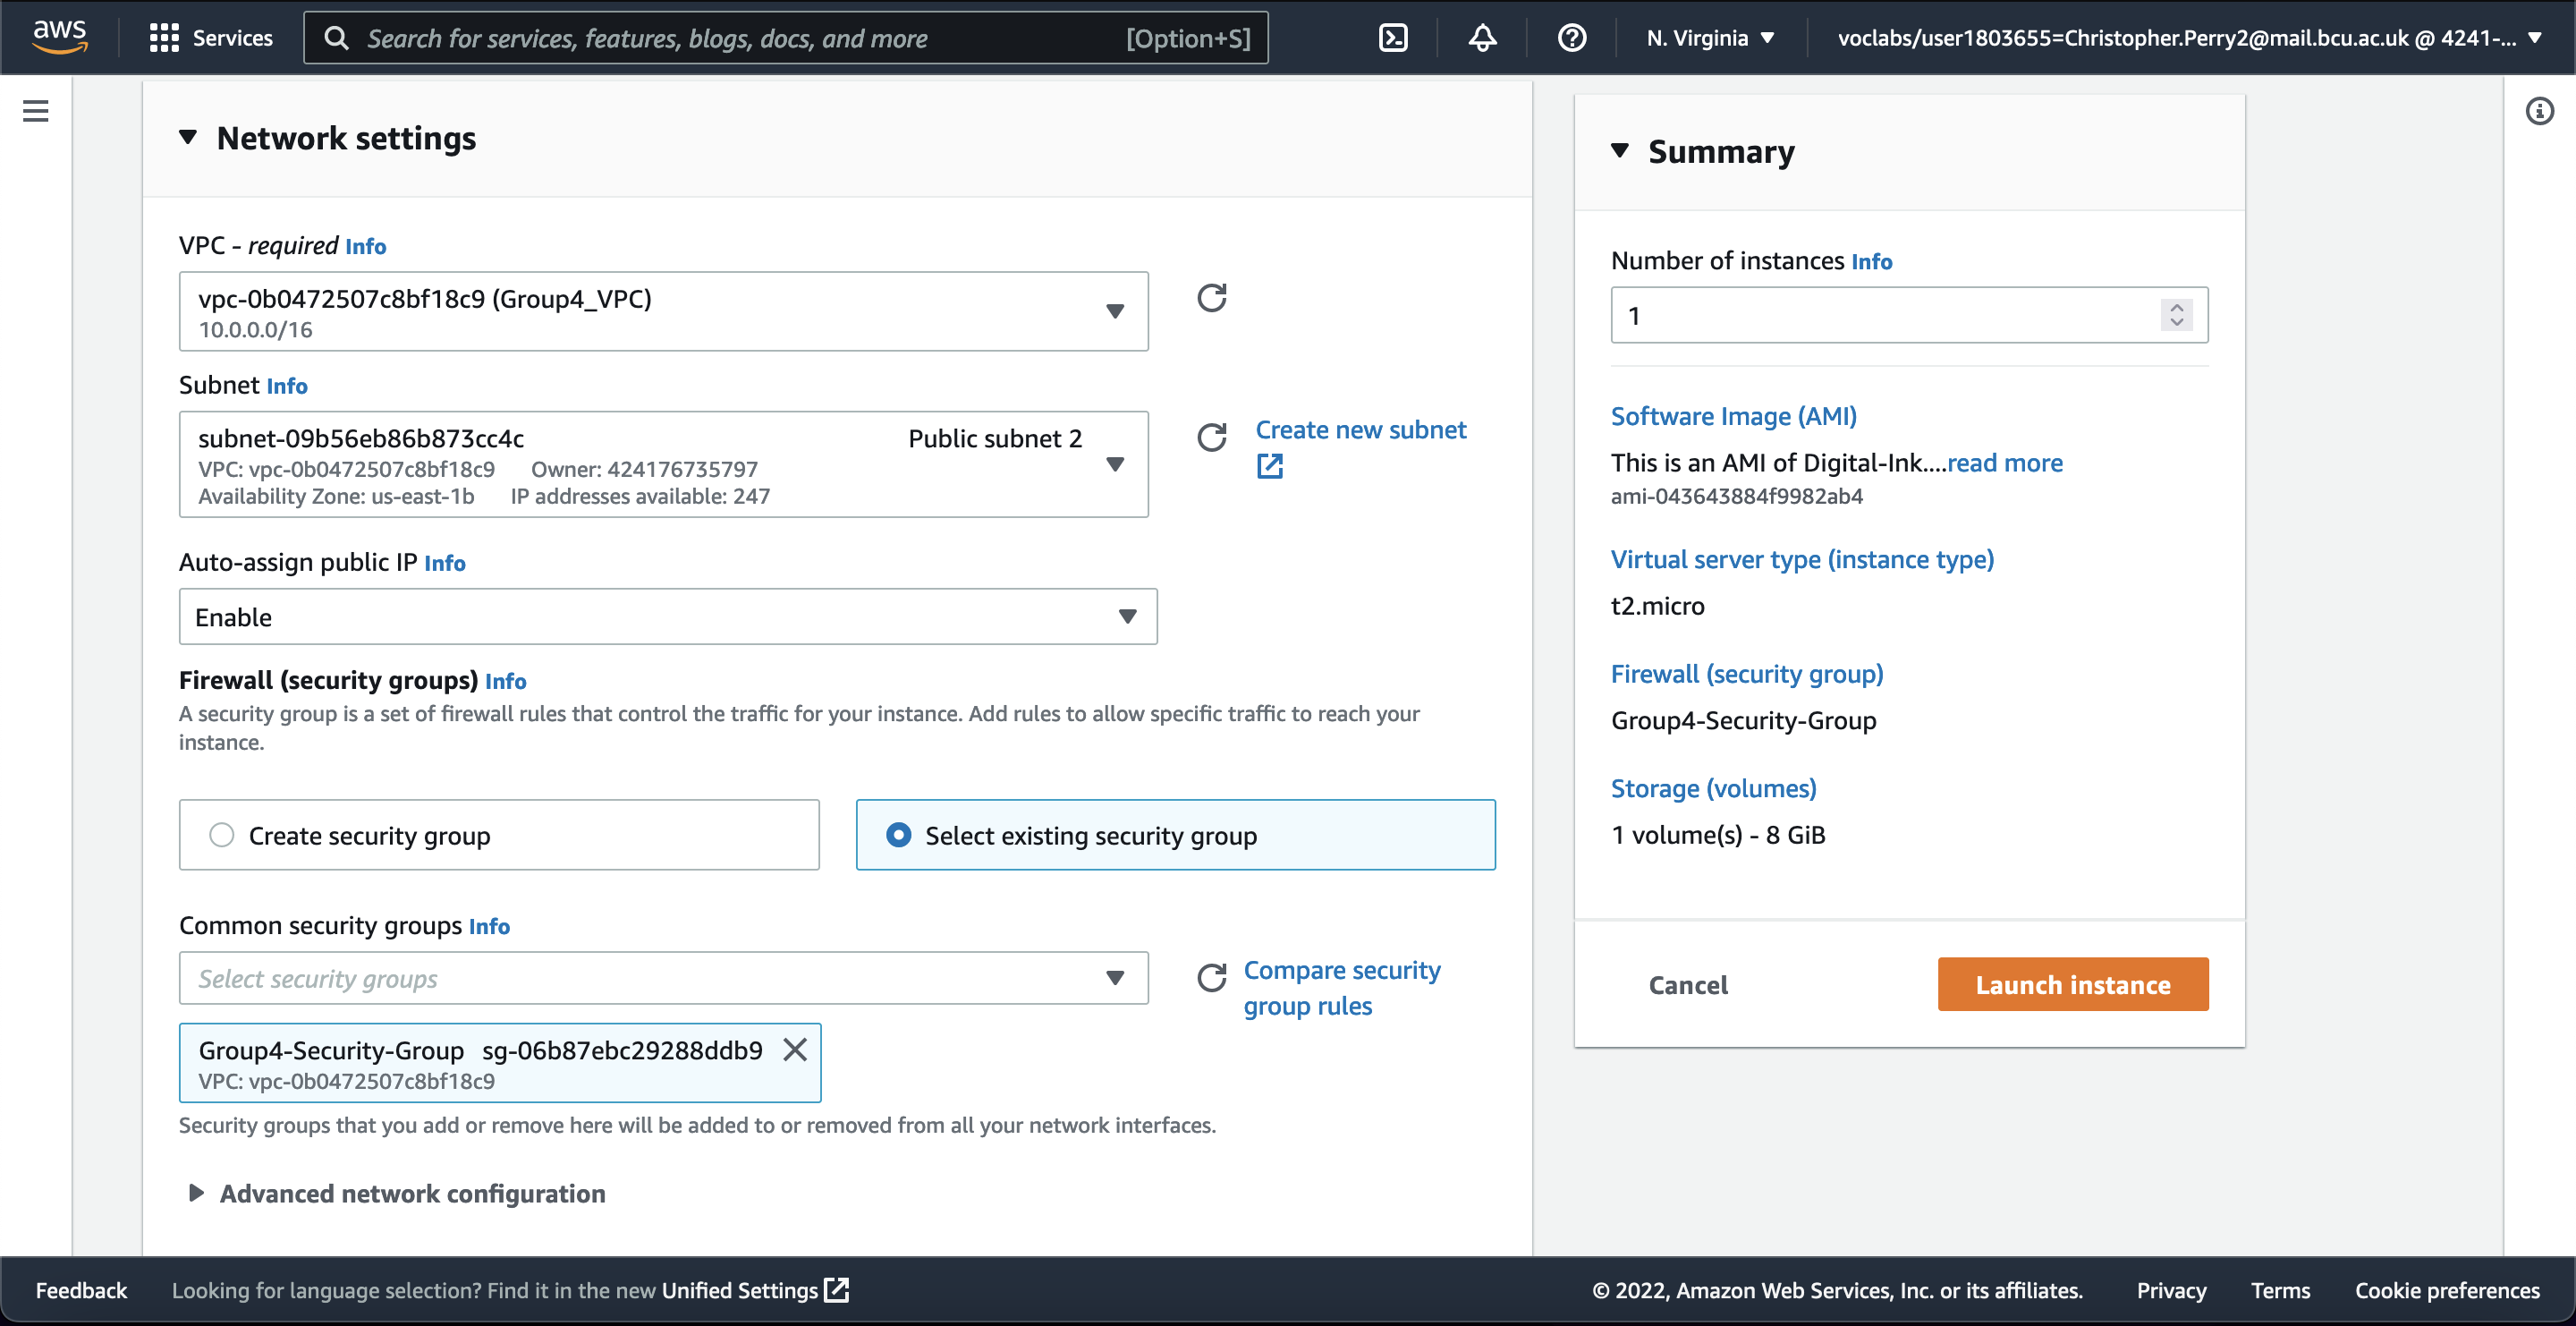
\includegraphics[width=\textwidth]{resources/elb/elb-instance-2-network-settings.png}
    \caption{Elastic Load Balancing}
    \label{fig:elb-instance-2-network-setting}
\end{figure}
\begin{figure}[!htbp]
    \centering
    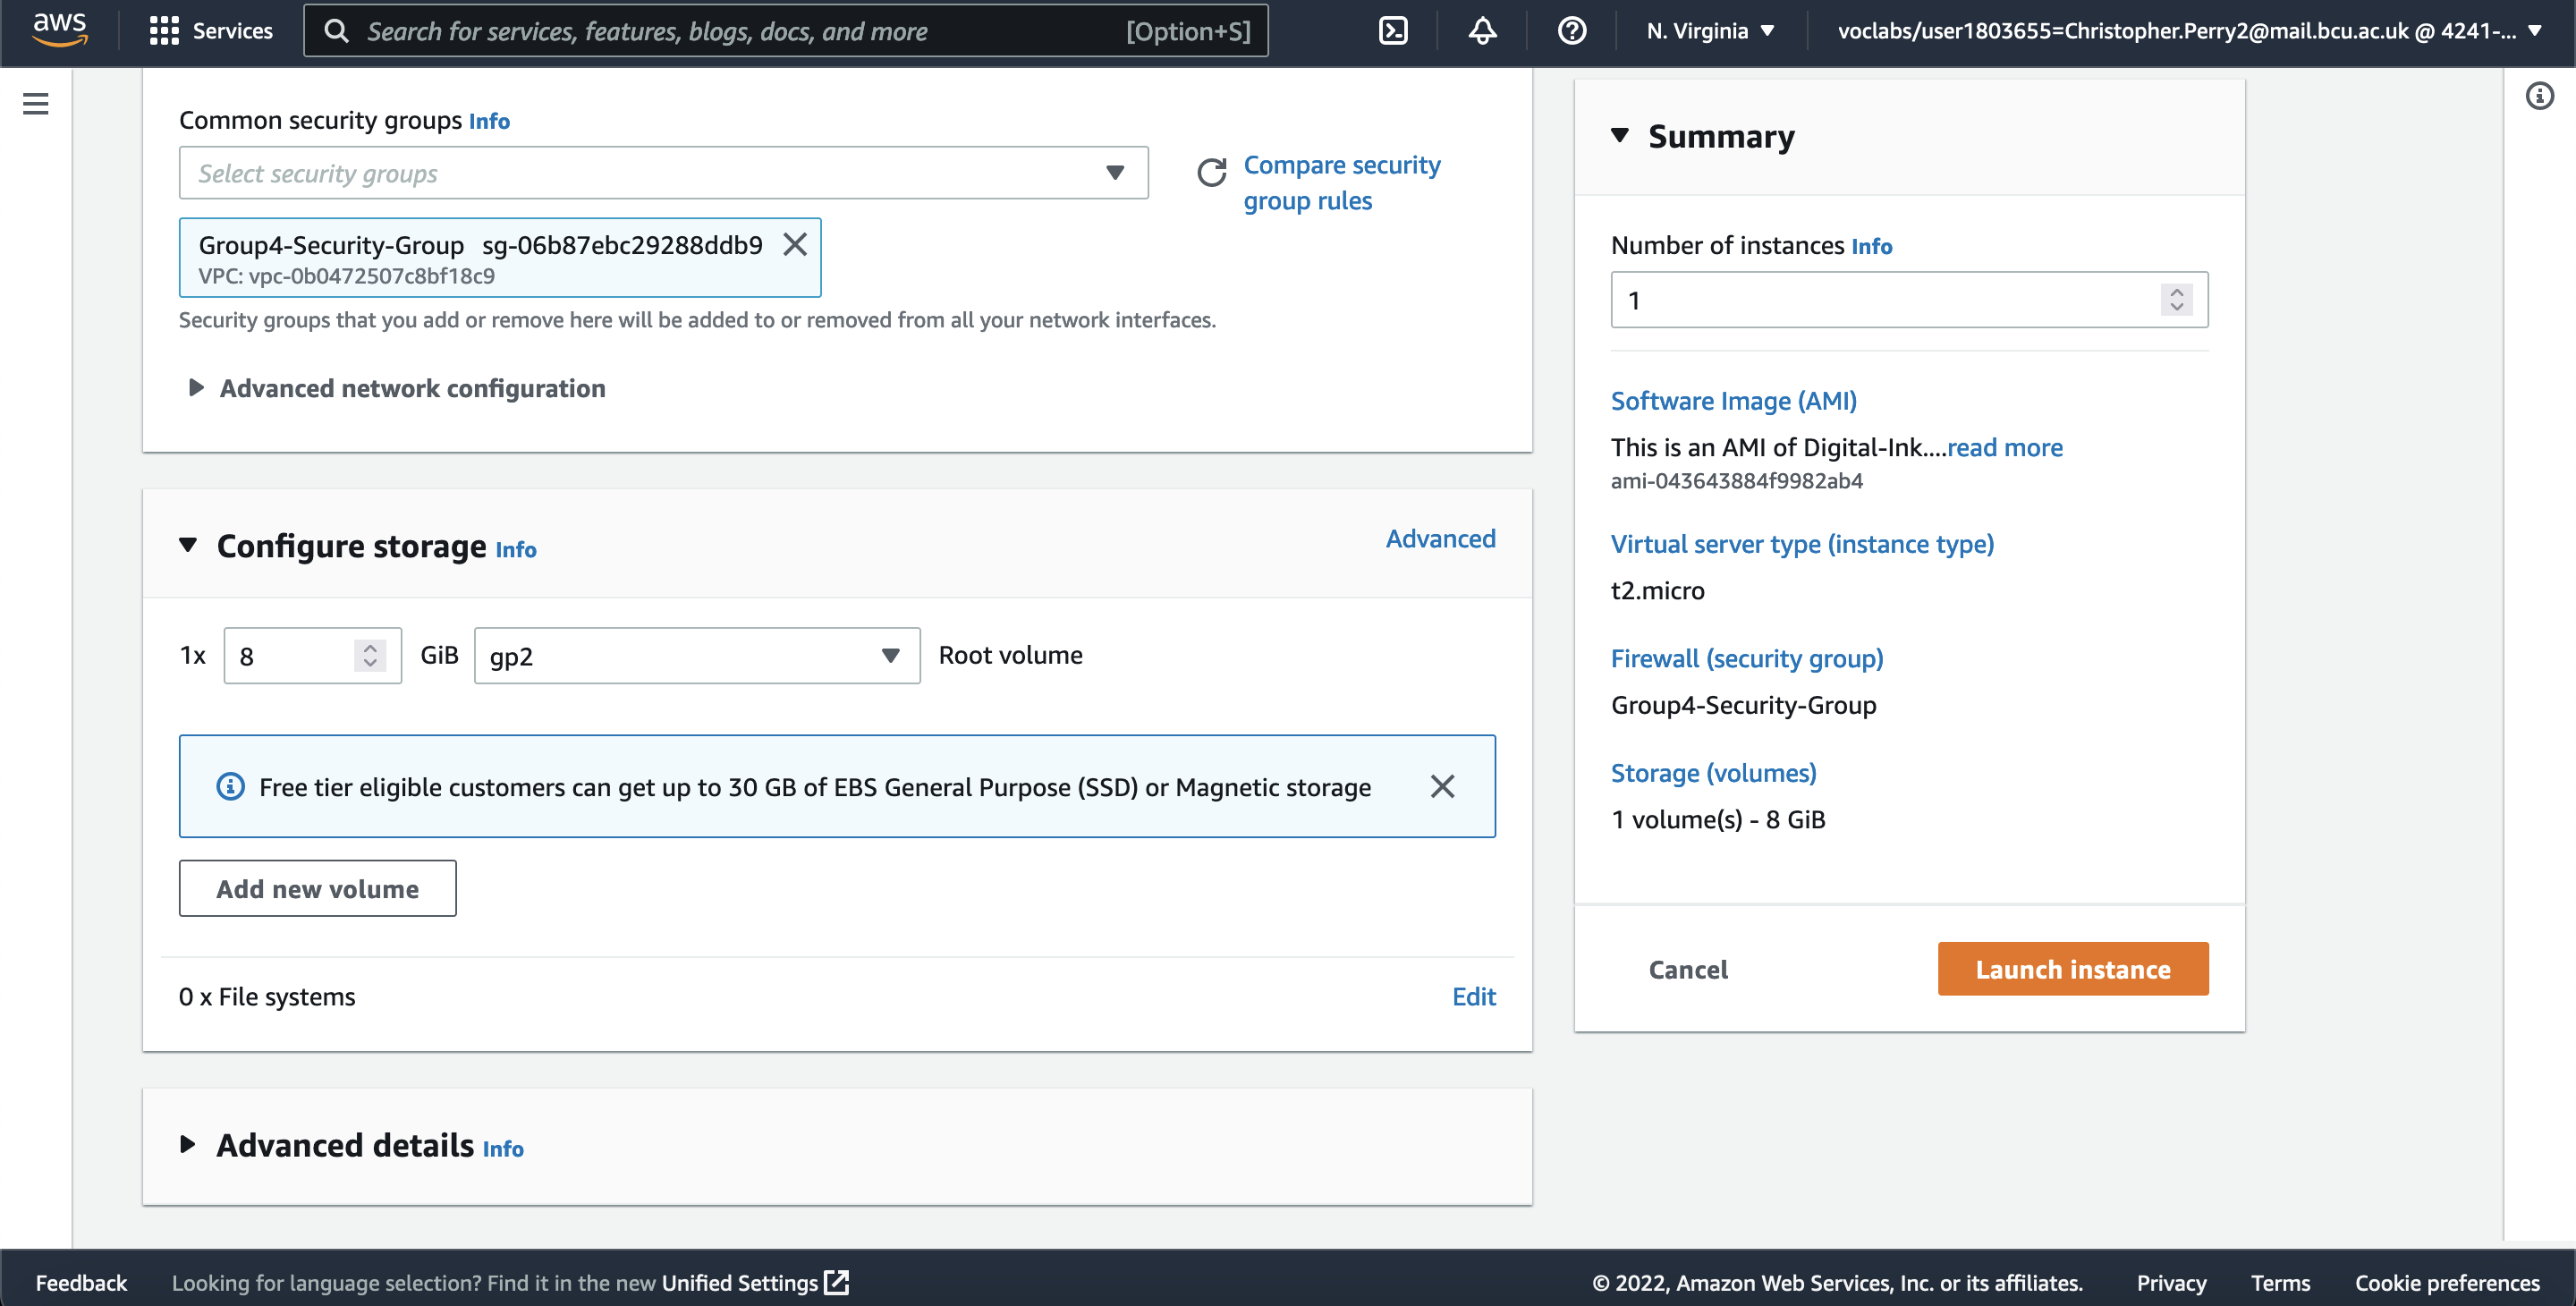
\includegraphics[width=\textwidth]{resources/elb/elb-instance-2-storage-config.png}
    \caption{Elastic Load Balancing}
    \label{fig:elb-instance-2-storage}
\end{figure}
\begin{figure}[!htbp]
    \centering
    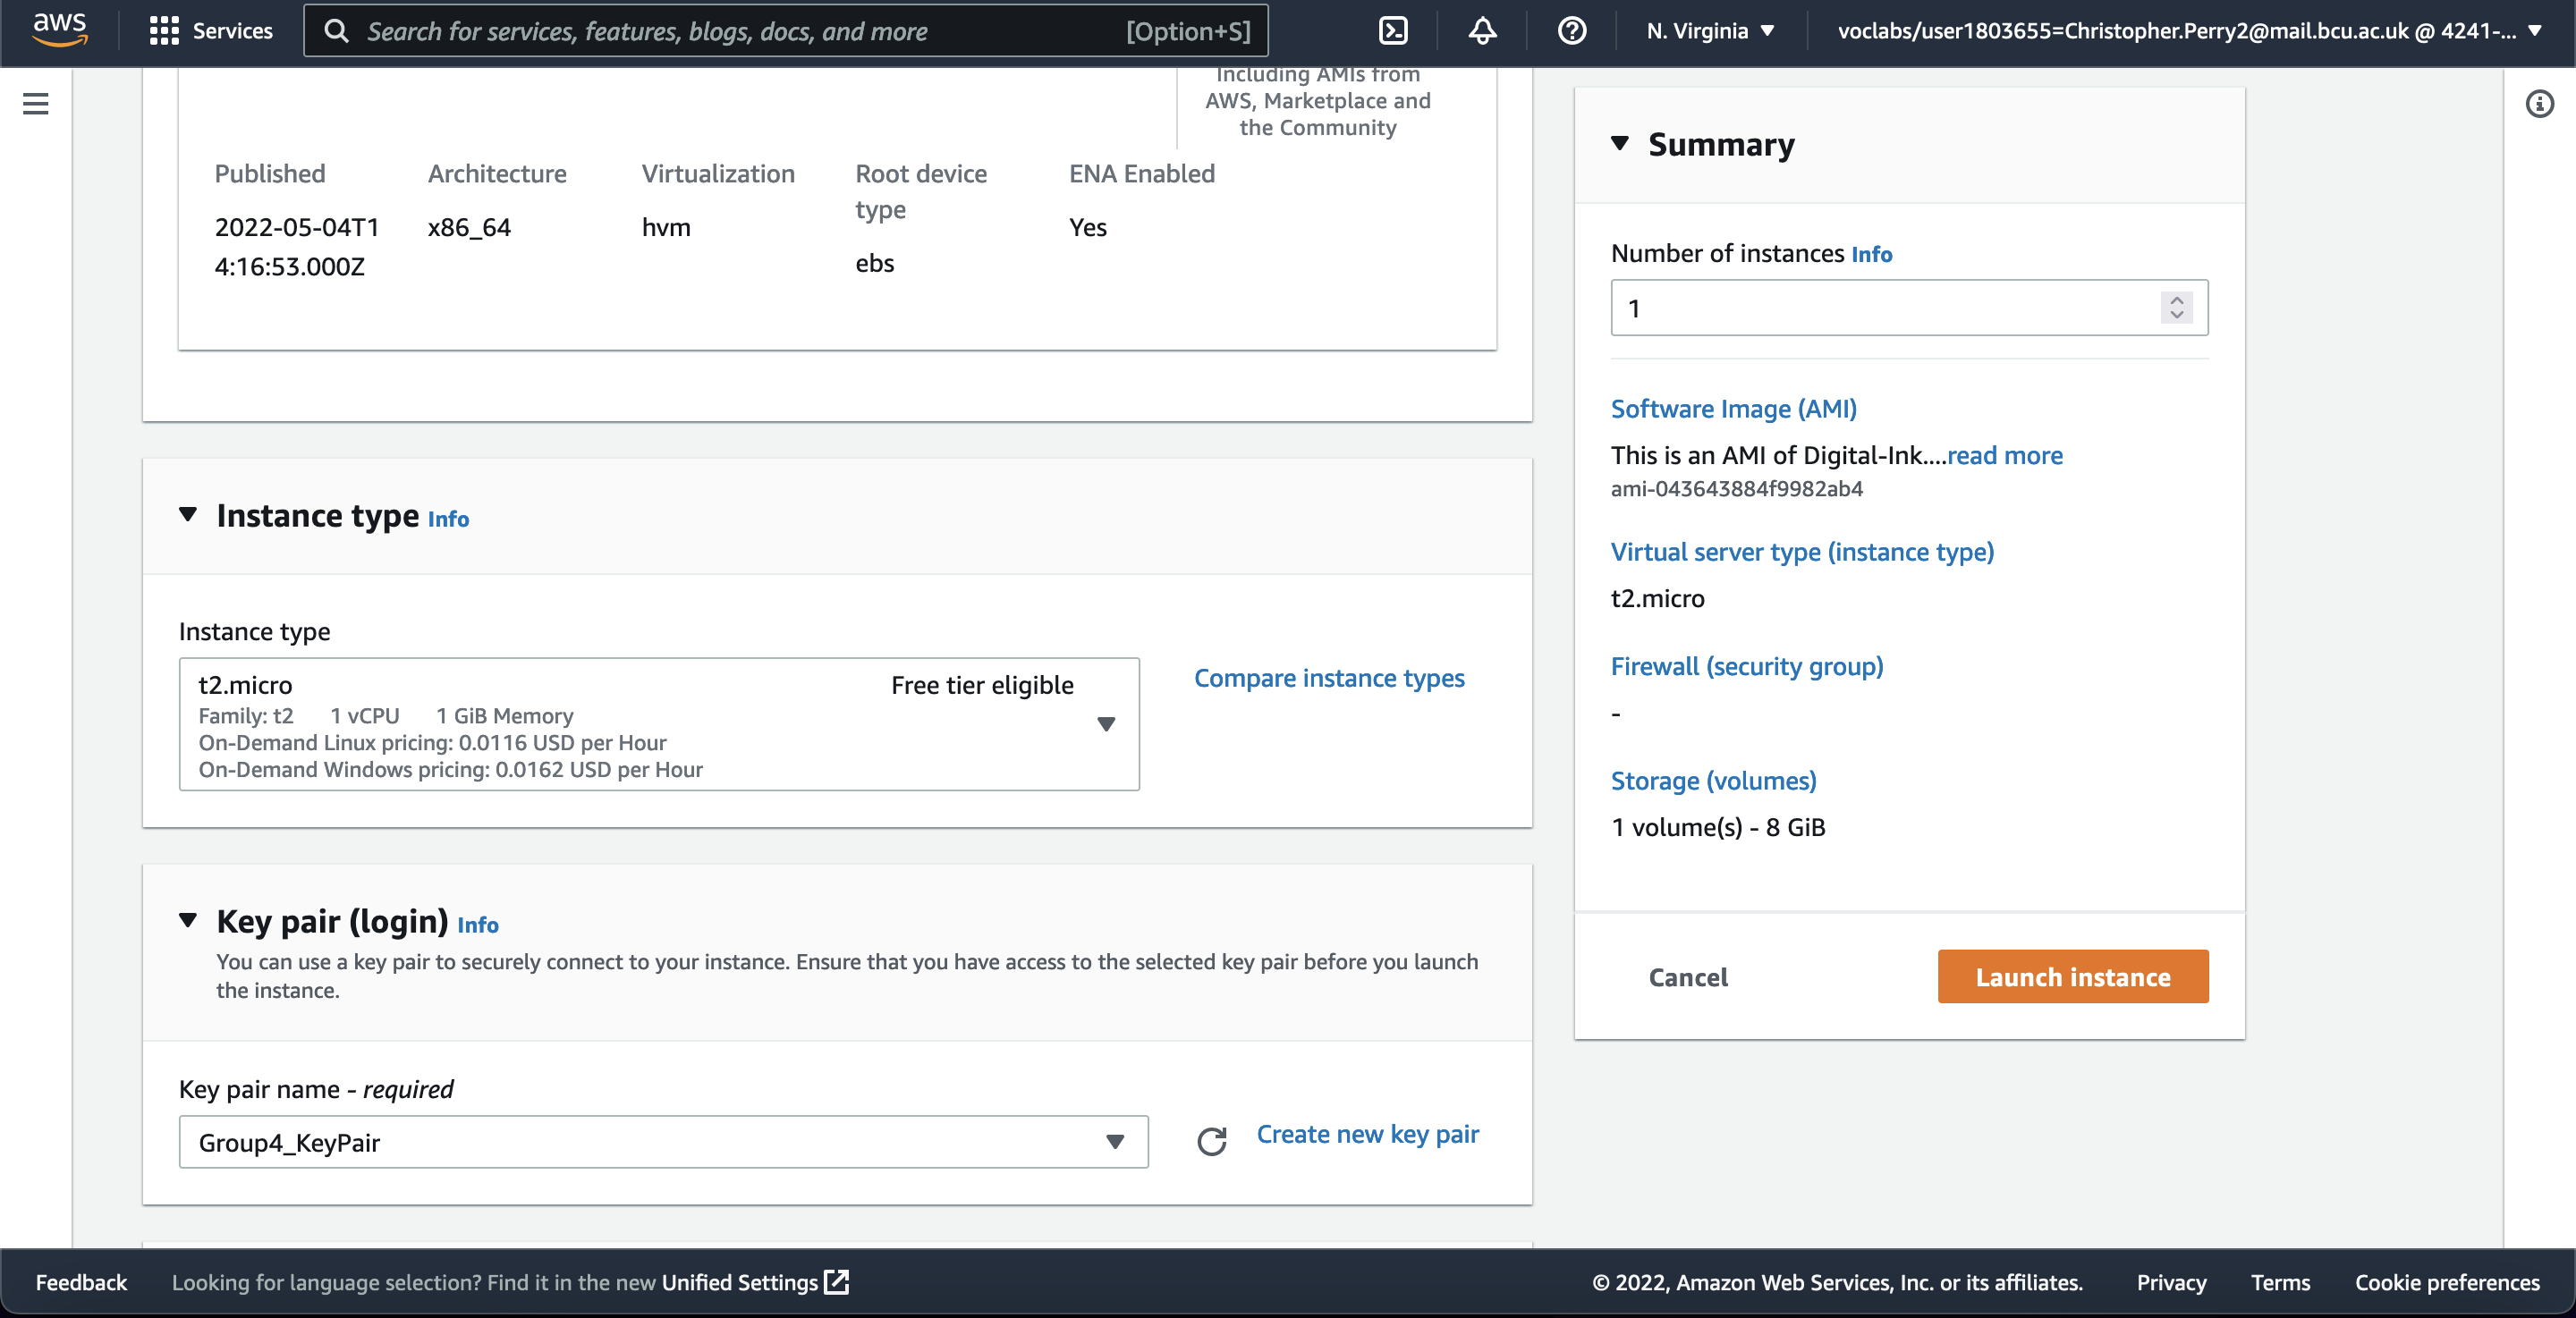
\includegraphics[width=\textwidth]{resources/elb/elb-instance-2-type-and-keypair.png}
    \caption{Elastic Load Balancing}
    \label{fig:elb-type-and-keypair}
\end{figure}
\begin{figure}[!htbp]
    \centering
    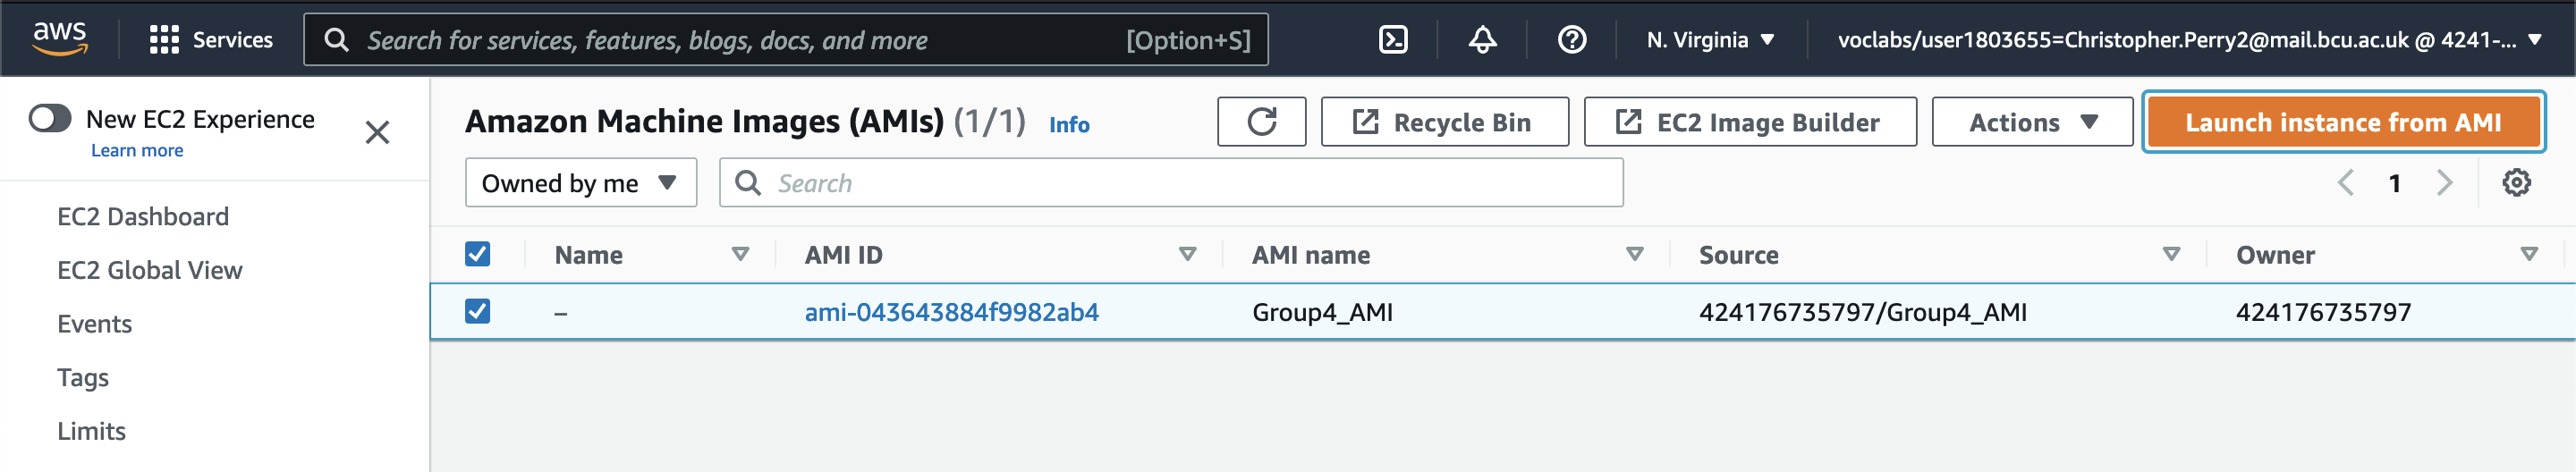
\includegraphics[width=\textwidth]{resources/elb/elb-instance-from-ami.png}
    \caption{Elastic Load Balancing}
    \label{fig:elb-instance-from-ami}
\end{figure}
\begin{figure}[!htbp]
    \centering
    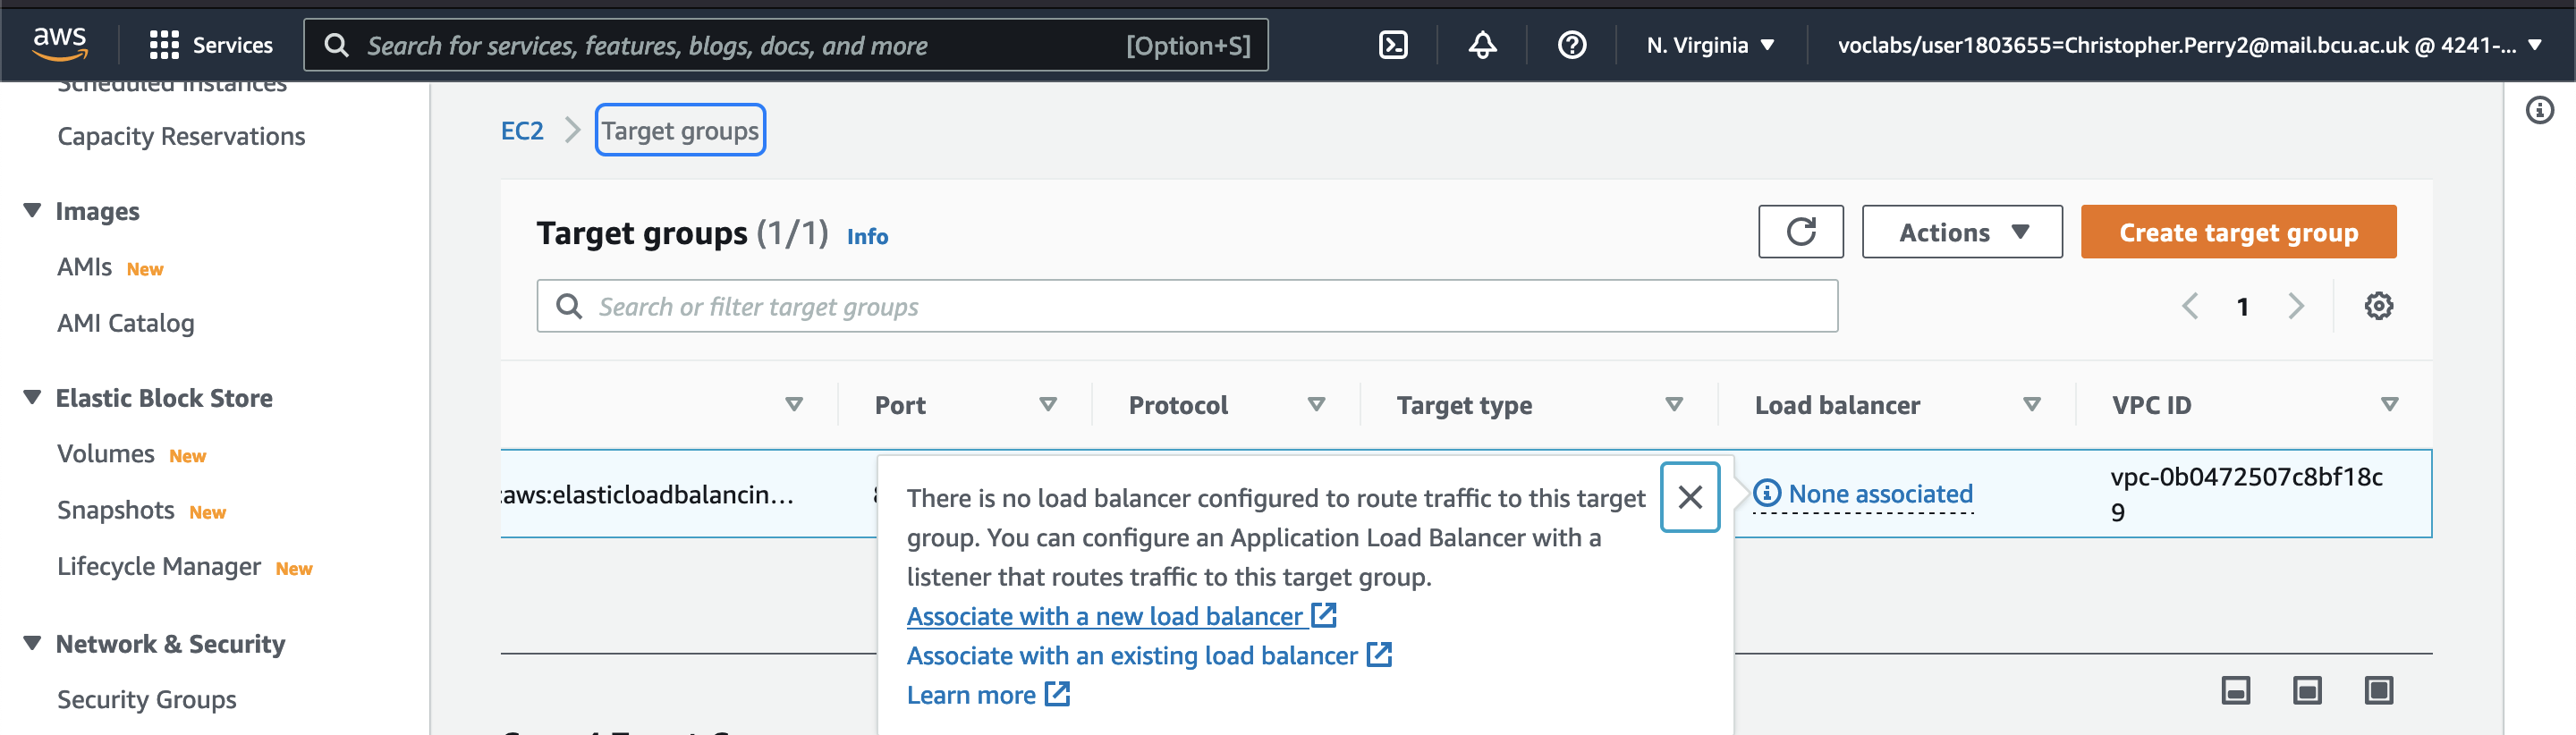
\includegraphics[width=\textwidth]{resources/elb/elb-load-balancer-creation.png}
    \caption{Elastic Load Balancing}
    \label{fig:elb-load-bal-create}
\end{figure}
\begin{figure}[!htbp]
    \centering
    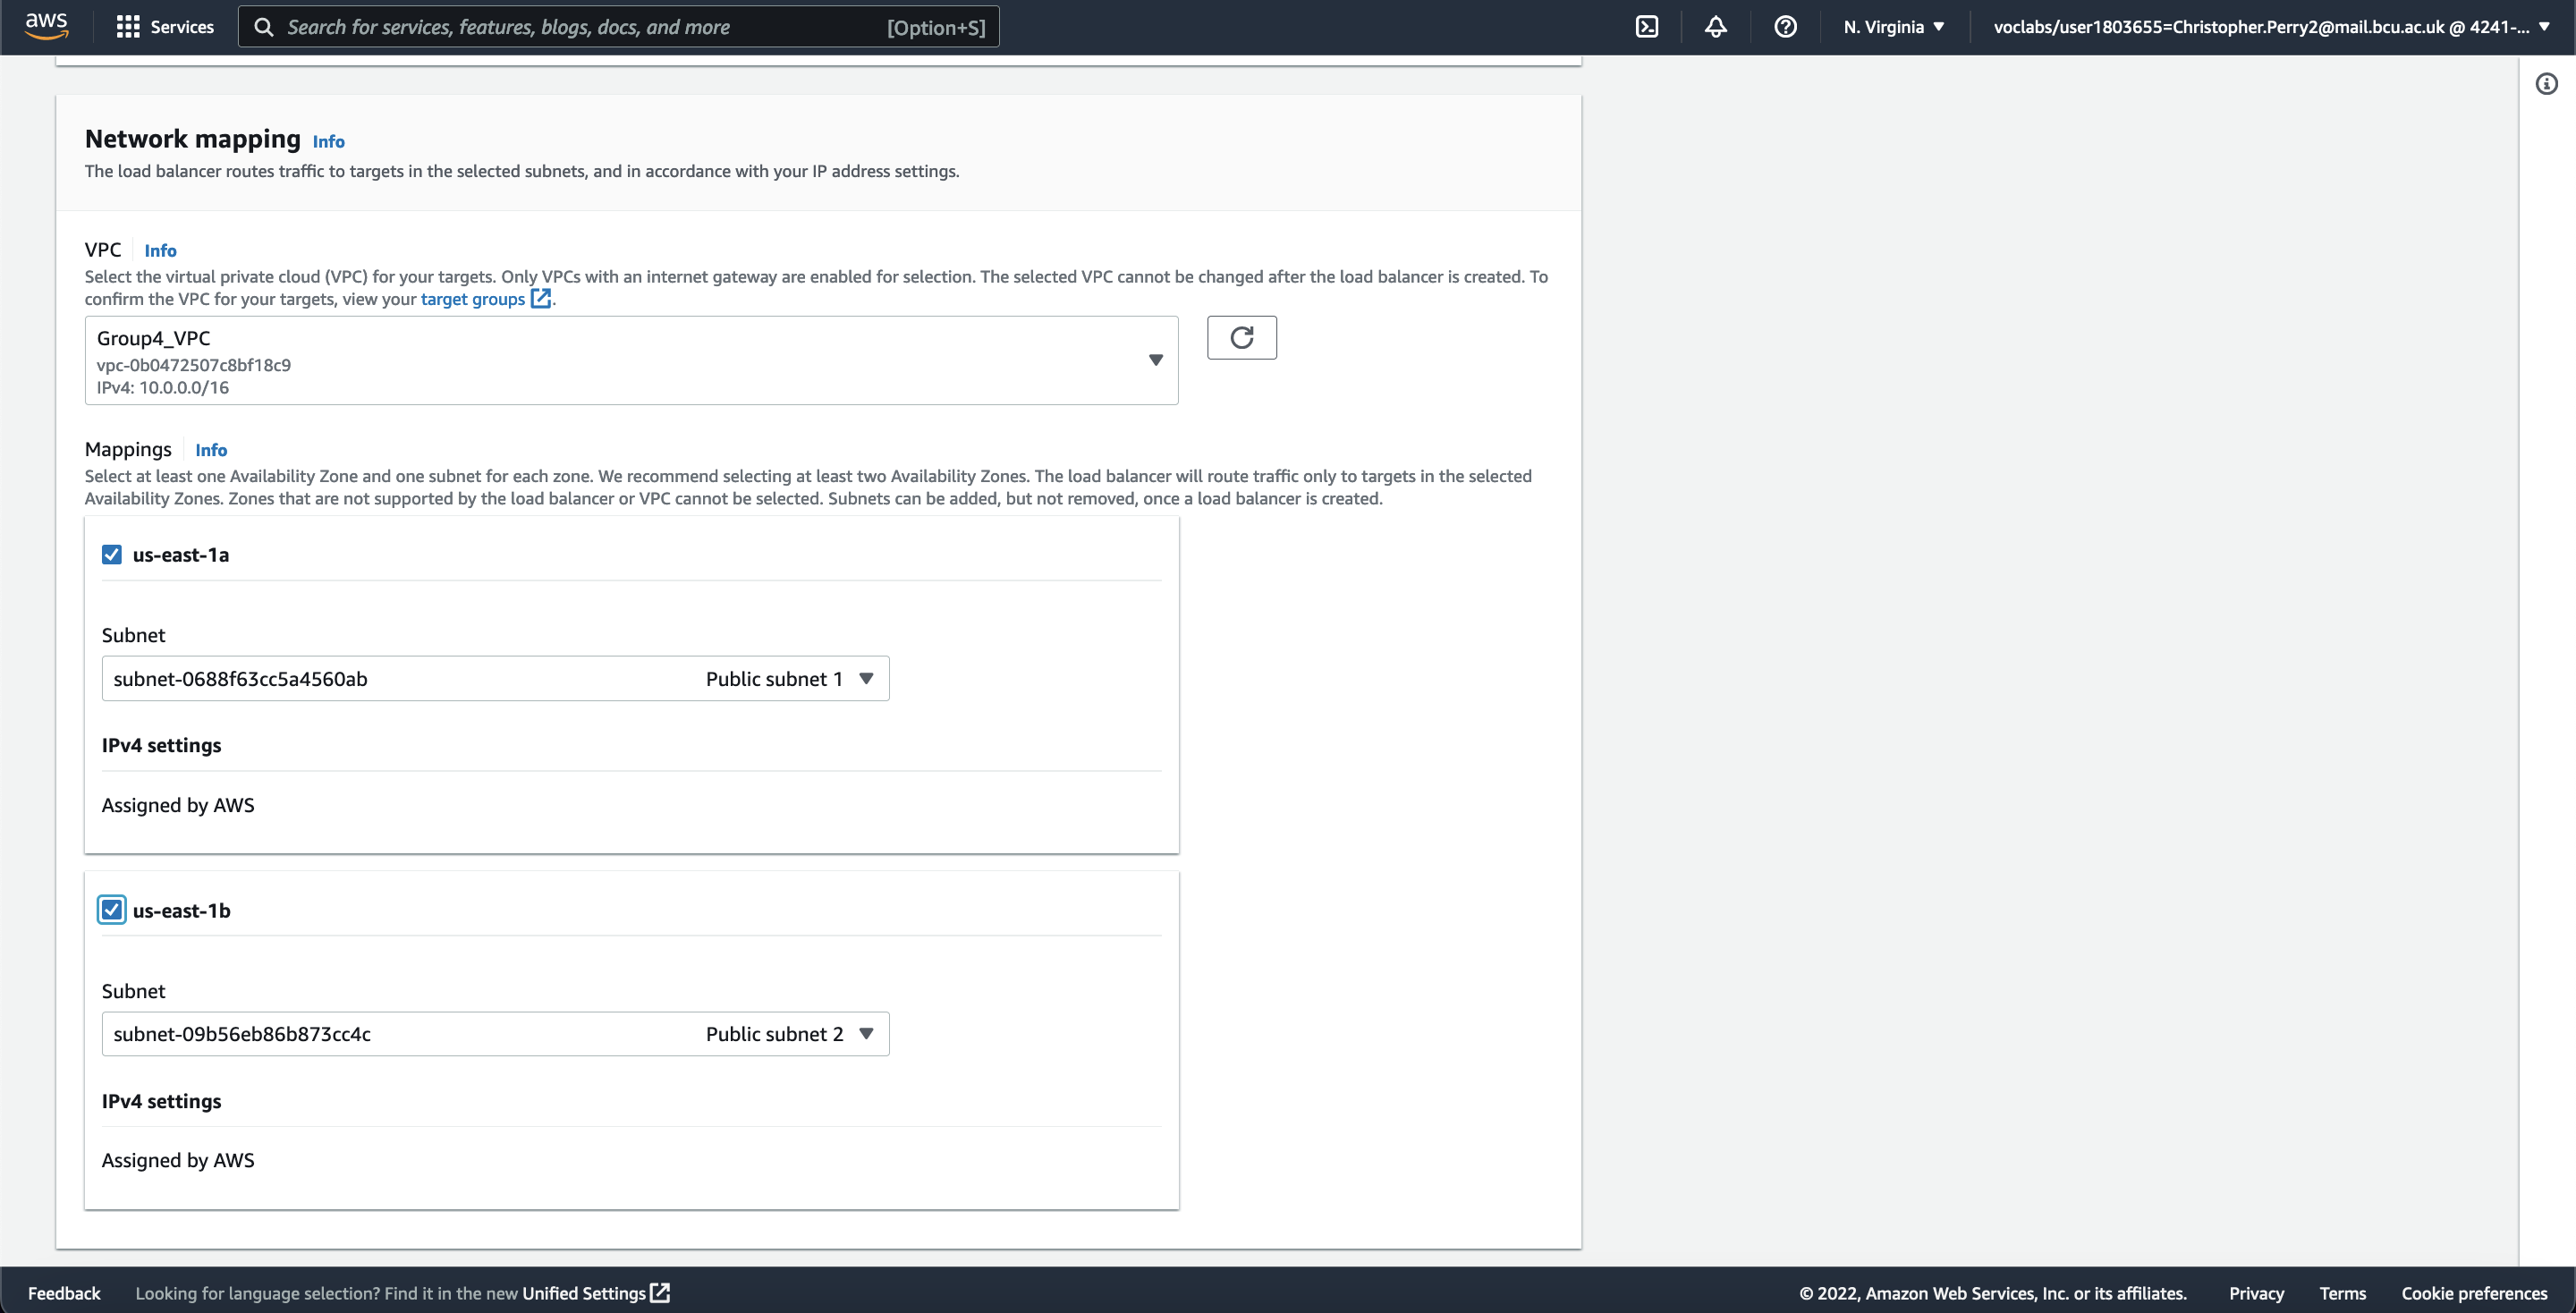
\includegraphics[width=\textwidth]{resources/elb/elb-network-mapping.png}
    \caption{Elastic Load Balancing}
    \label{fig:elb-networ-mapping}
\end{figure}
\begin{figure}[!htbp]
    \centering
    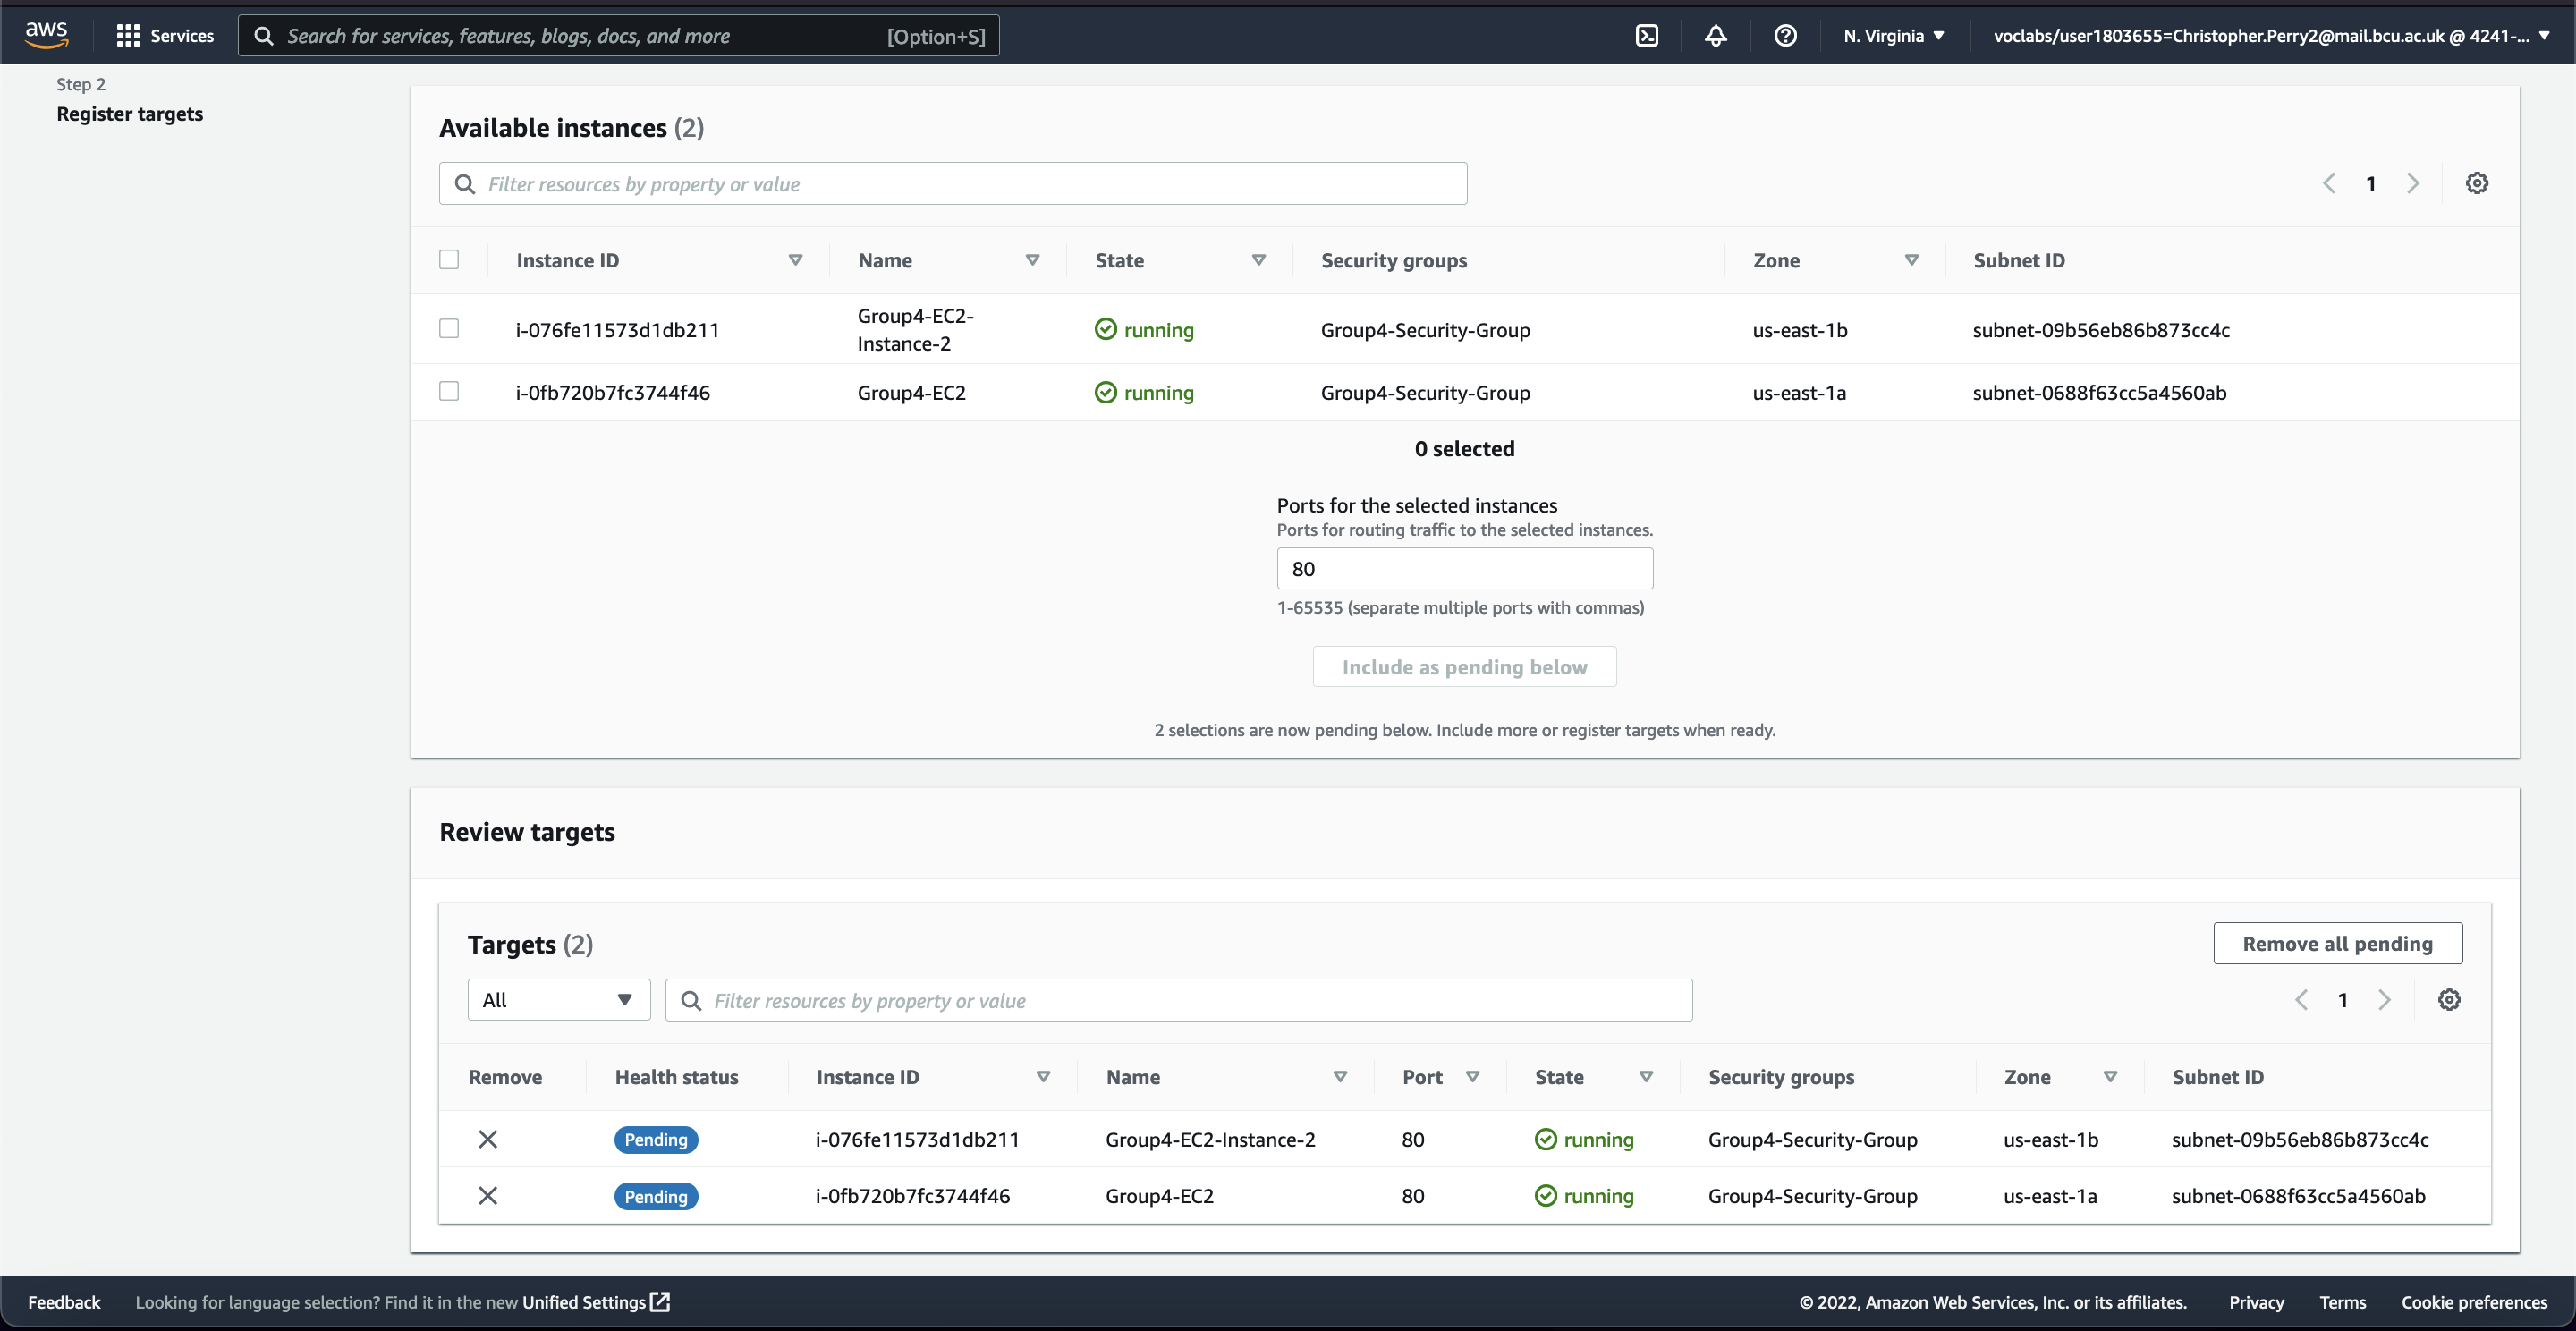
\includegraphics[width=\textwidth]{resources/elb/elb-register-targets.png}
    \caption{Elastic Load Balancing}
    \label{fig:elb-register-targets}
\end{figure}
\begin{figure}[!htbp]
    \centering
    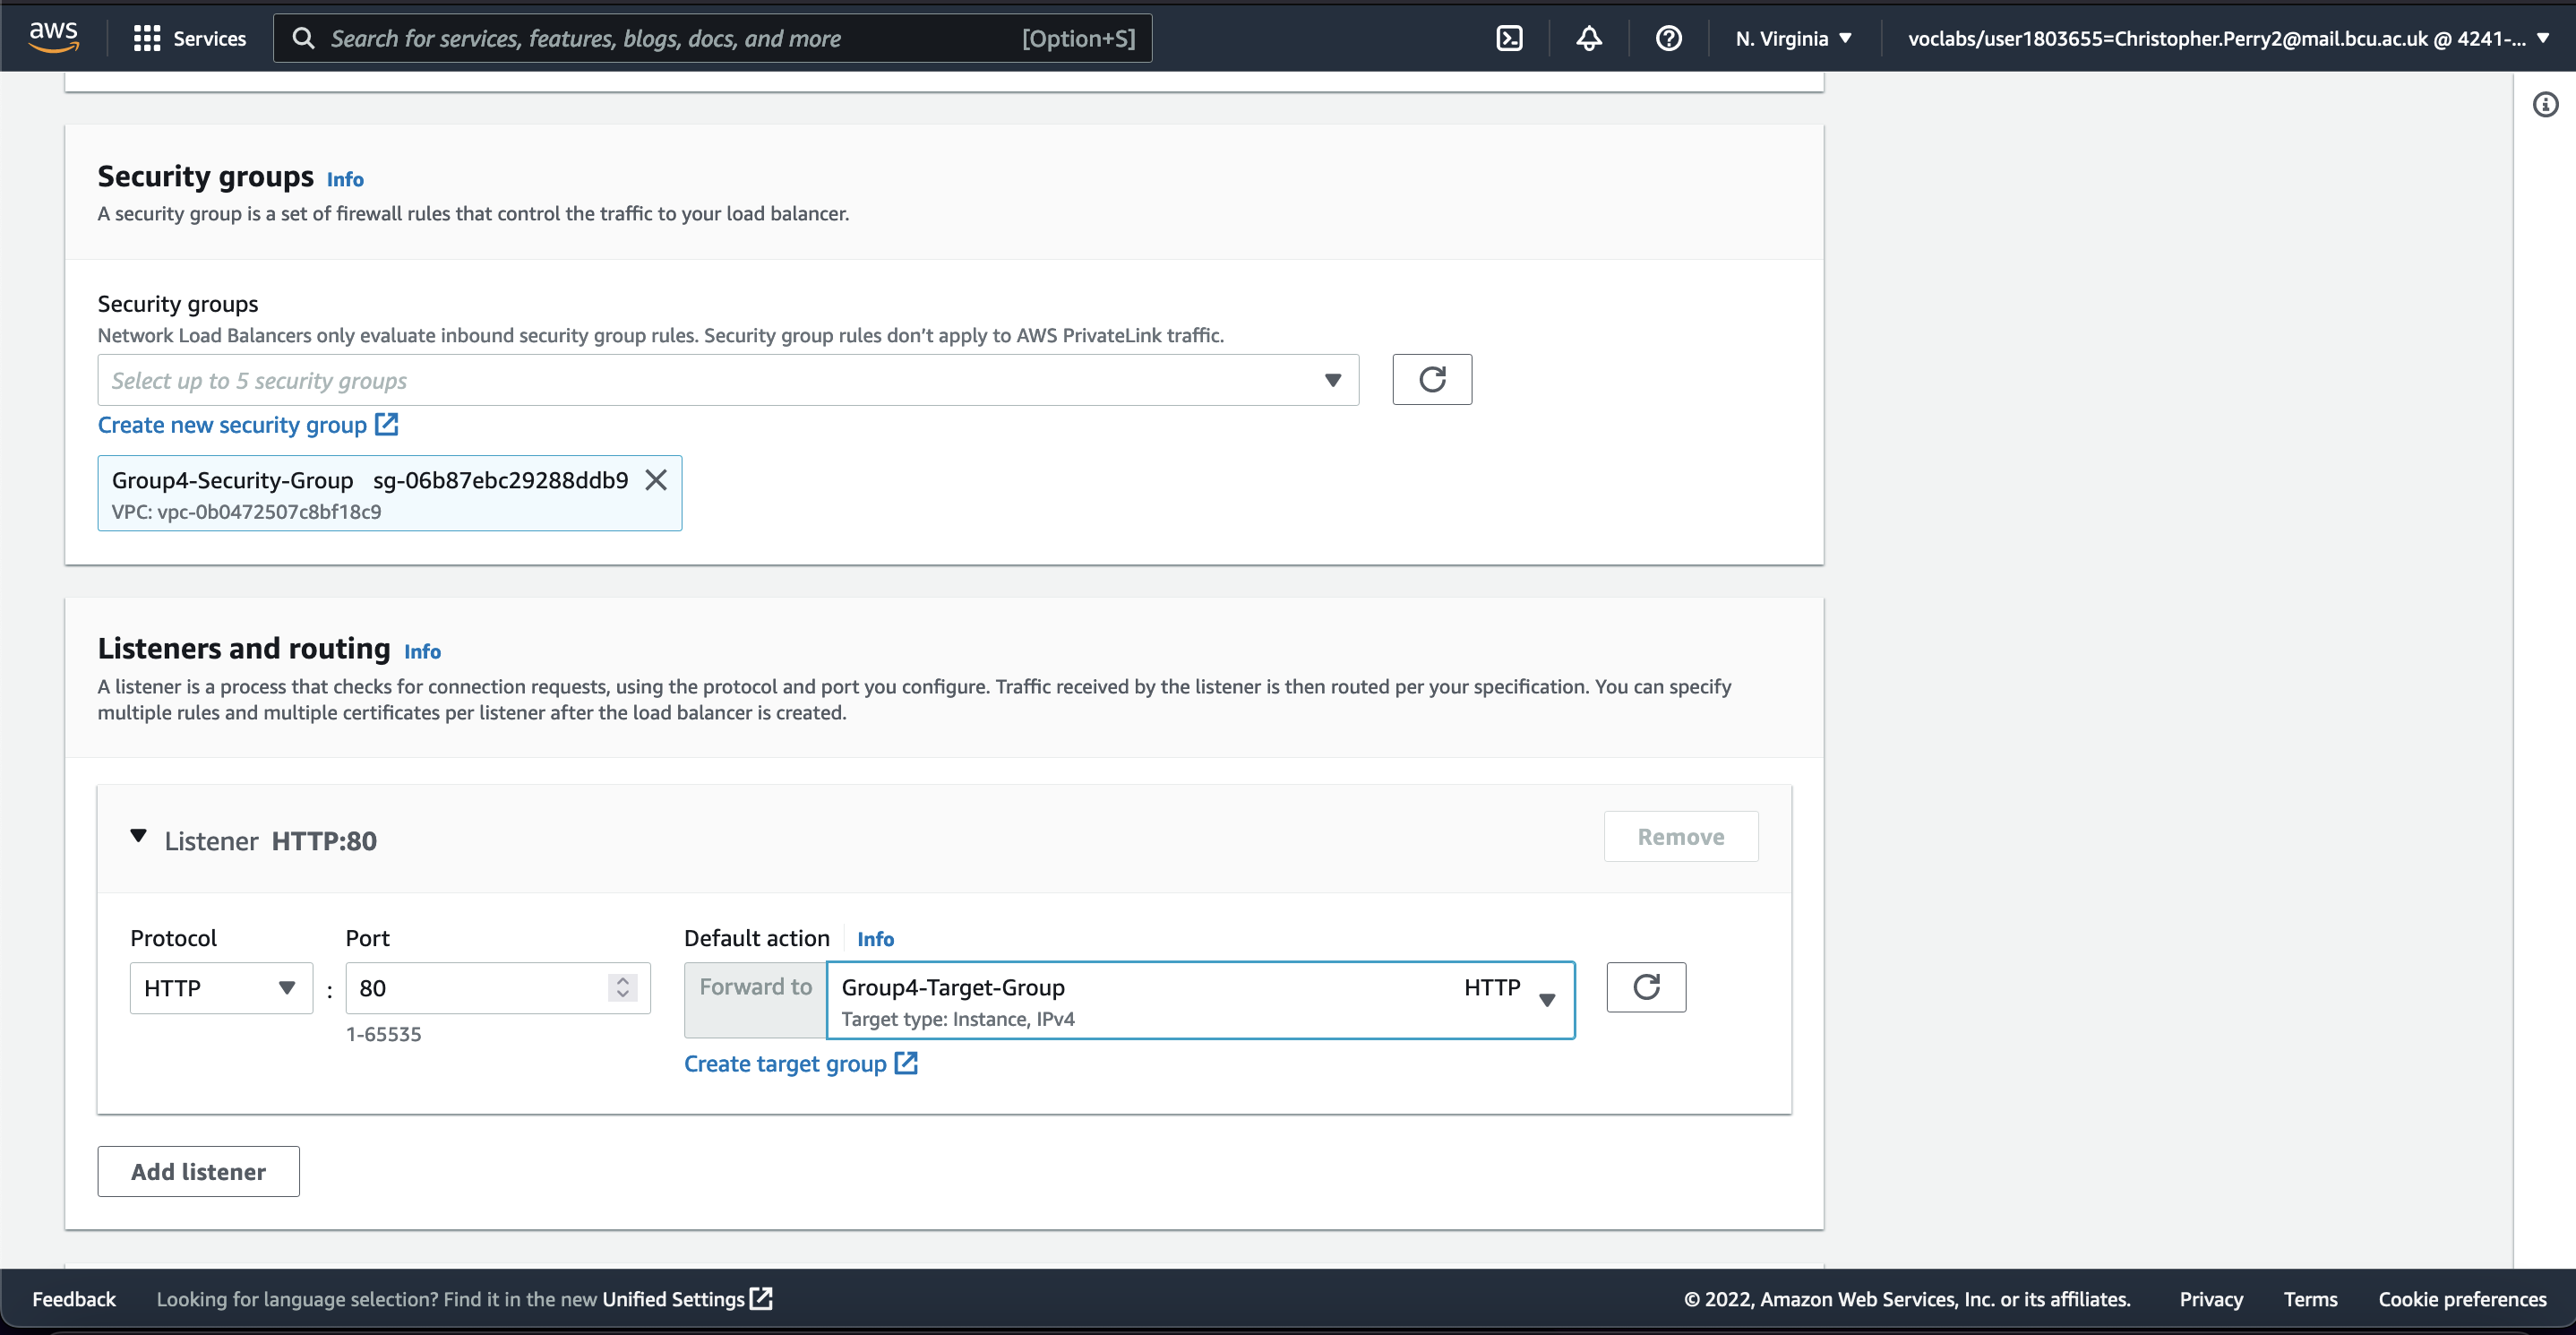
\includegraphics[width=\textwidth]{resources/elb/elb-security-groups-and-listeners.png}
    \caption{Elastic Load Balancing}
    \label{fig:elb-security-groups}
\end{figure}
\begin{figure}[!htbp]
    \centering
    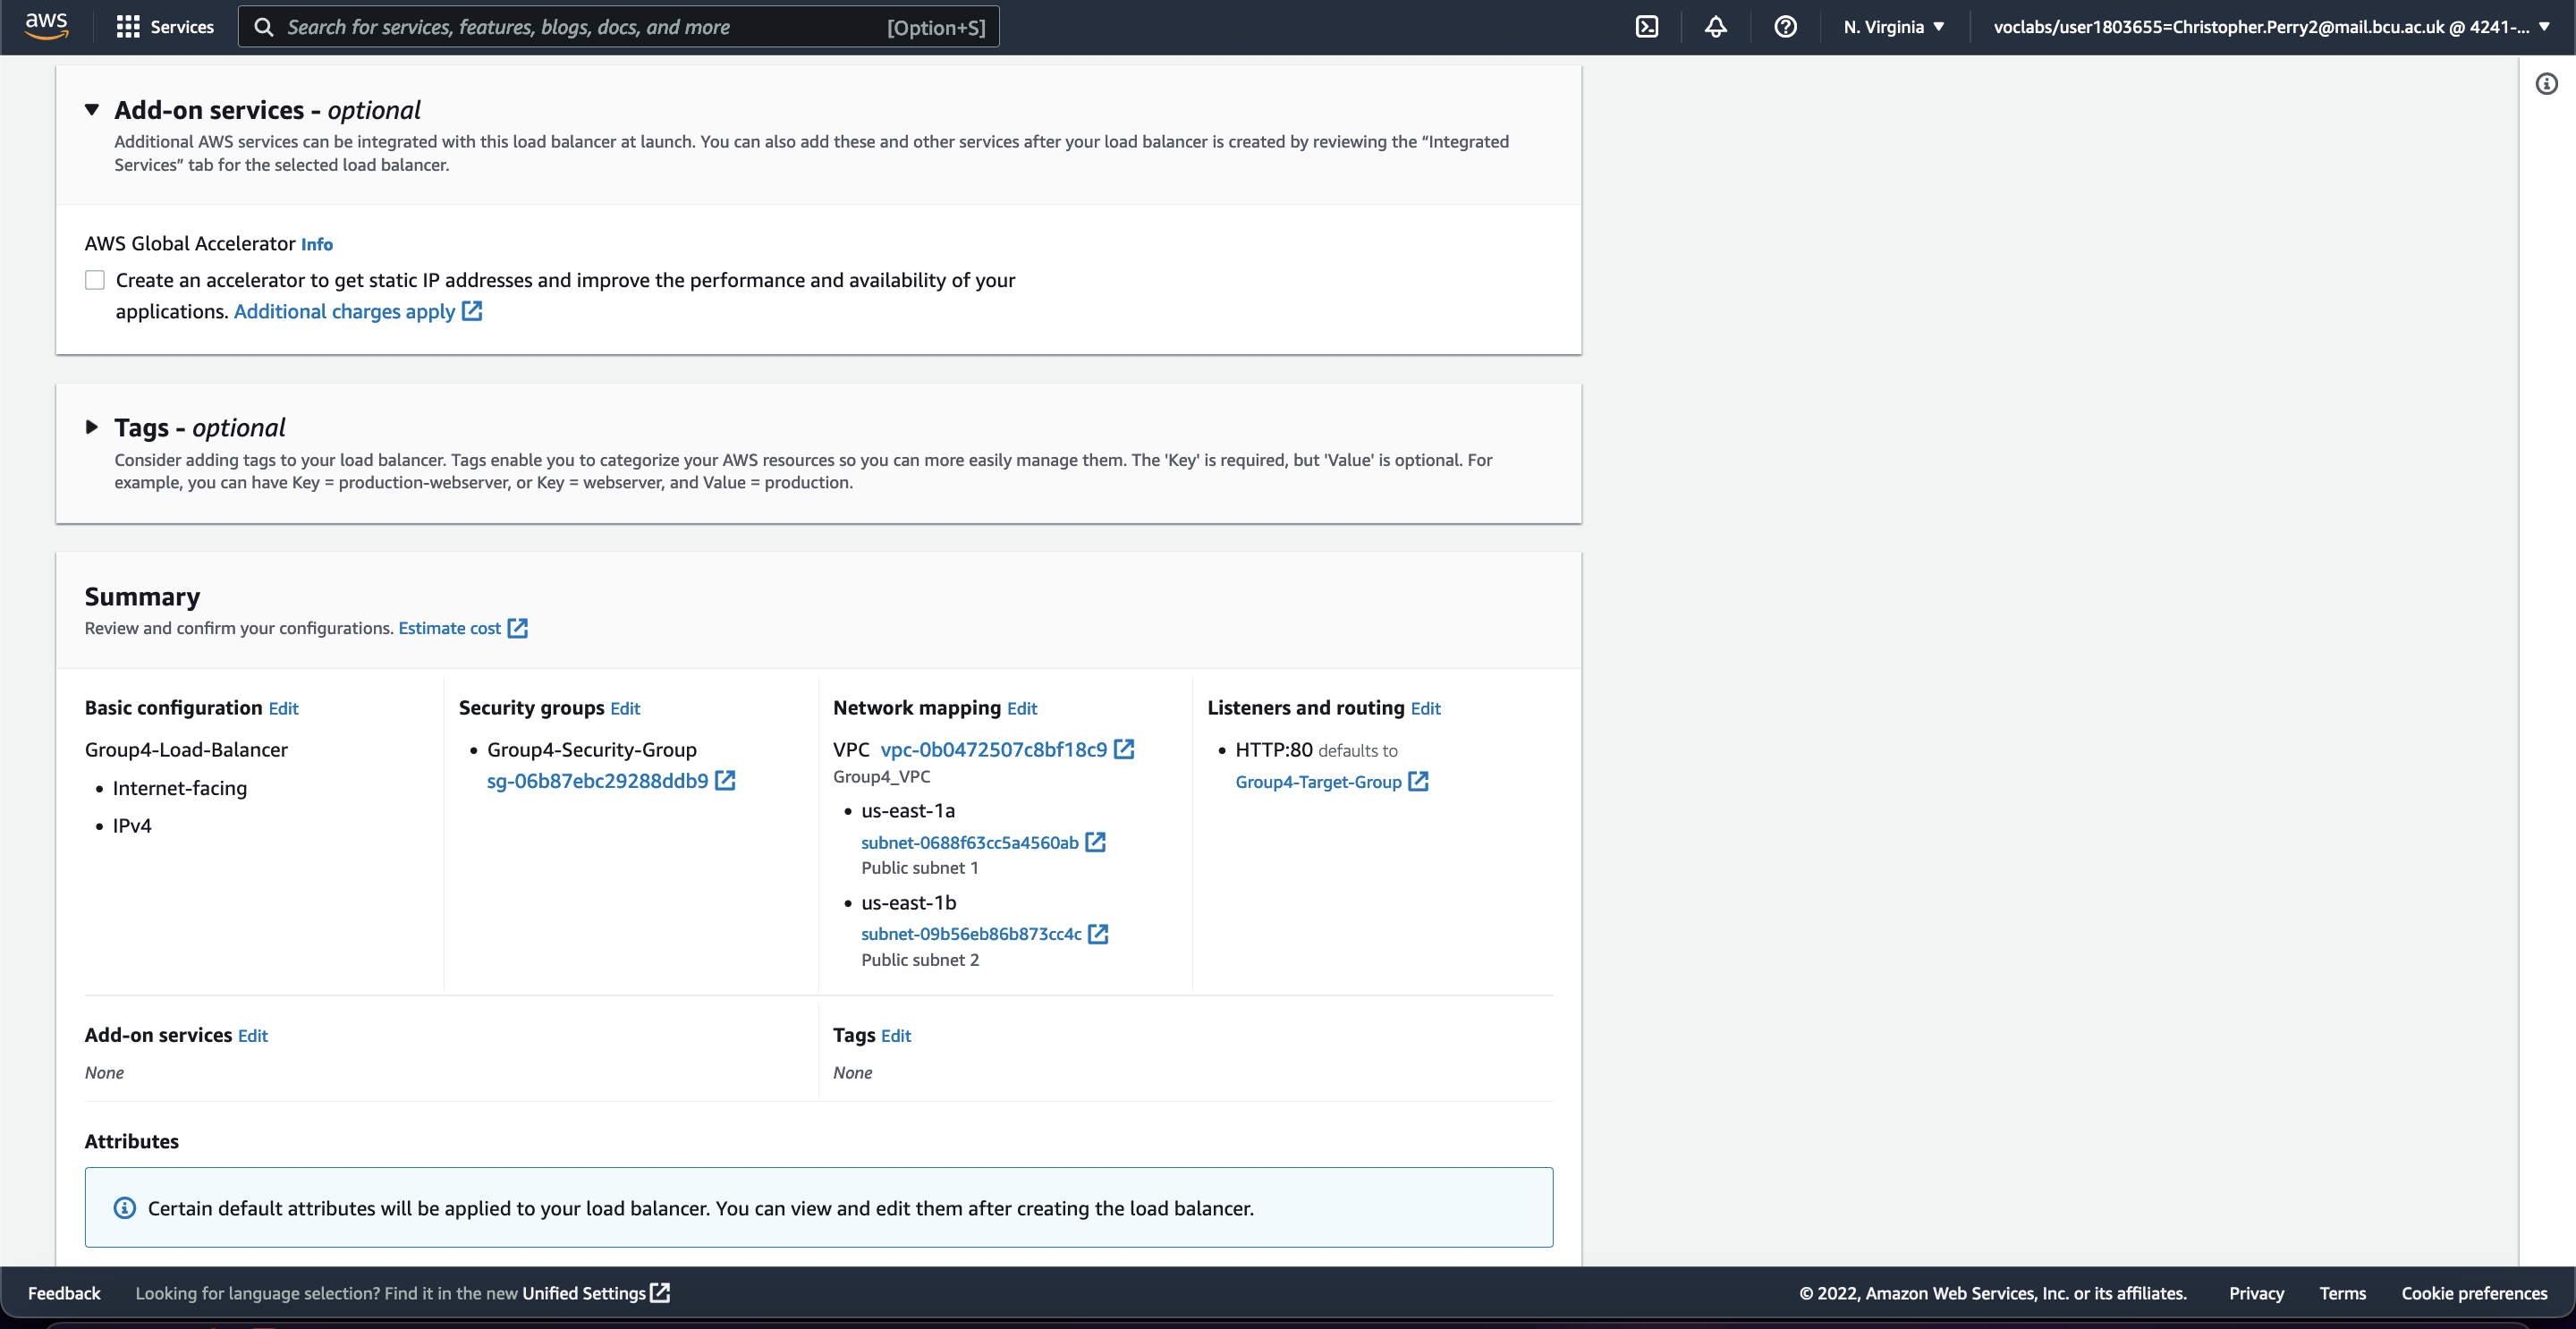
\includegraphics[width=\textwidth]{resources/elb/elb-summary.png}
    \caption{Elastic Load Balancing}
    \label{fig:elb-summary}
\end{figure}
\begin{figure}[!htbp]
    \centering
    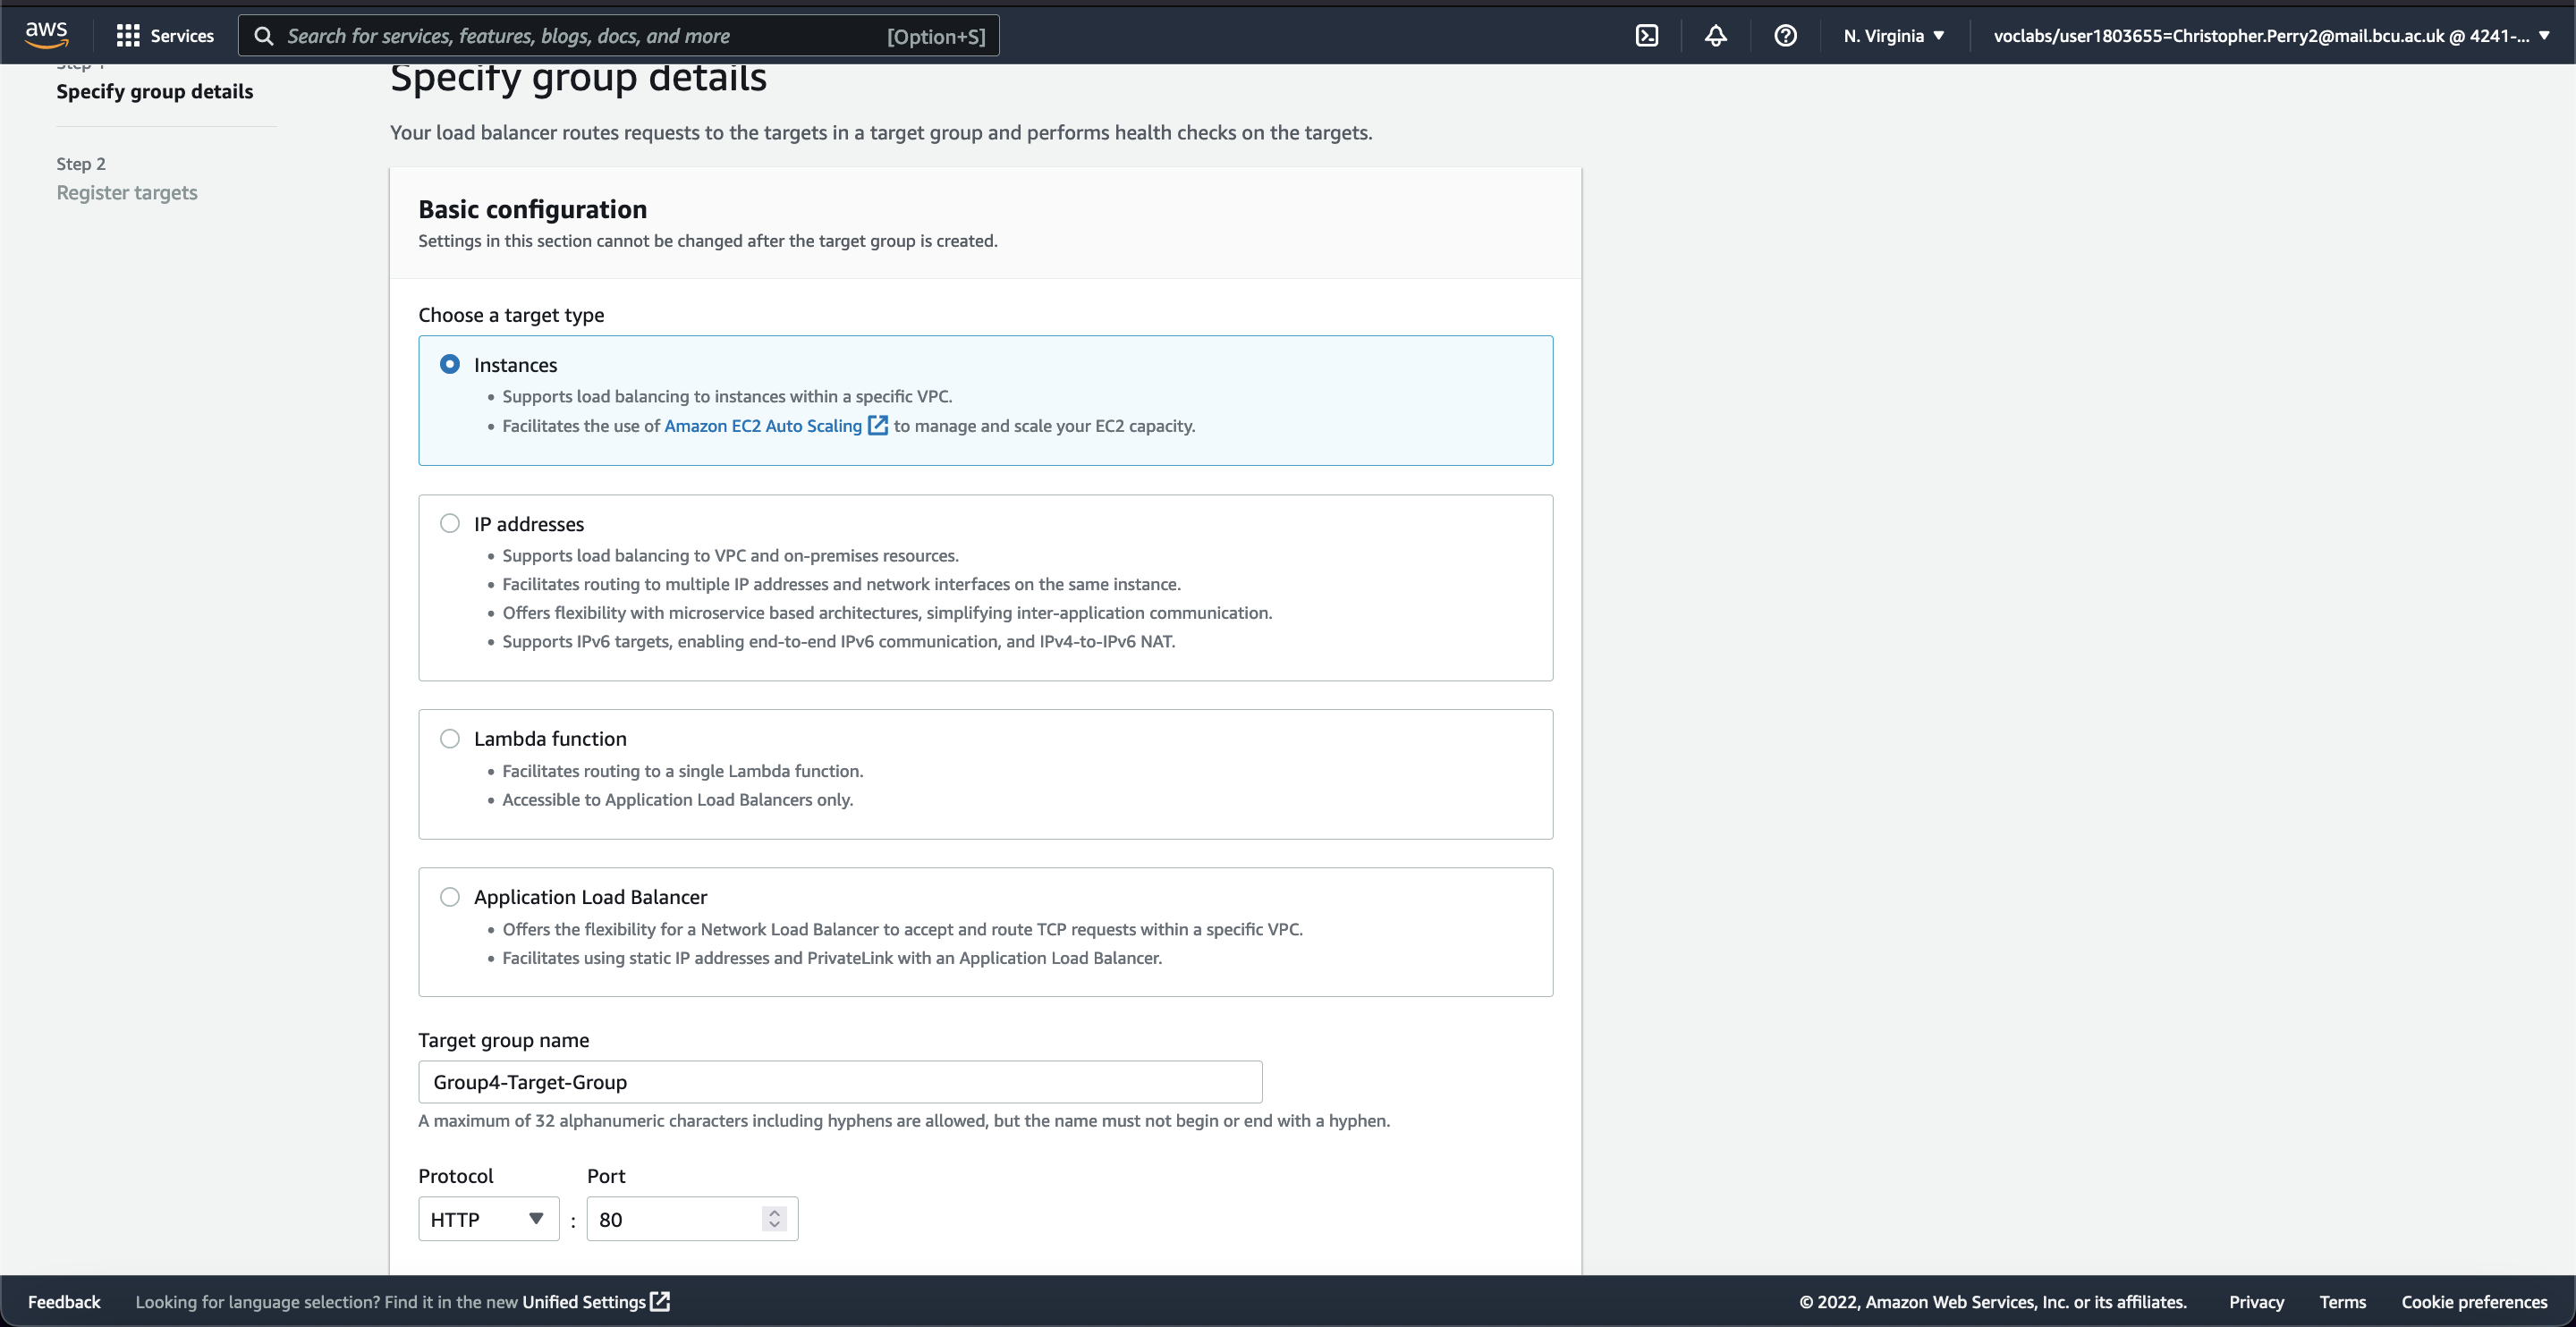
\includegraphics[width=\textwidth]{resources/elb/elb-target-group-basic-config.png}
    \caption{Elastic Load Balancing}
    \label{fig:elb-target-group-basic-config}
\end{figure}
\begin{figure}[!htbp]
    \centering
    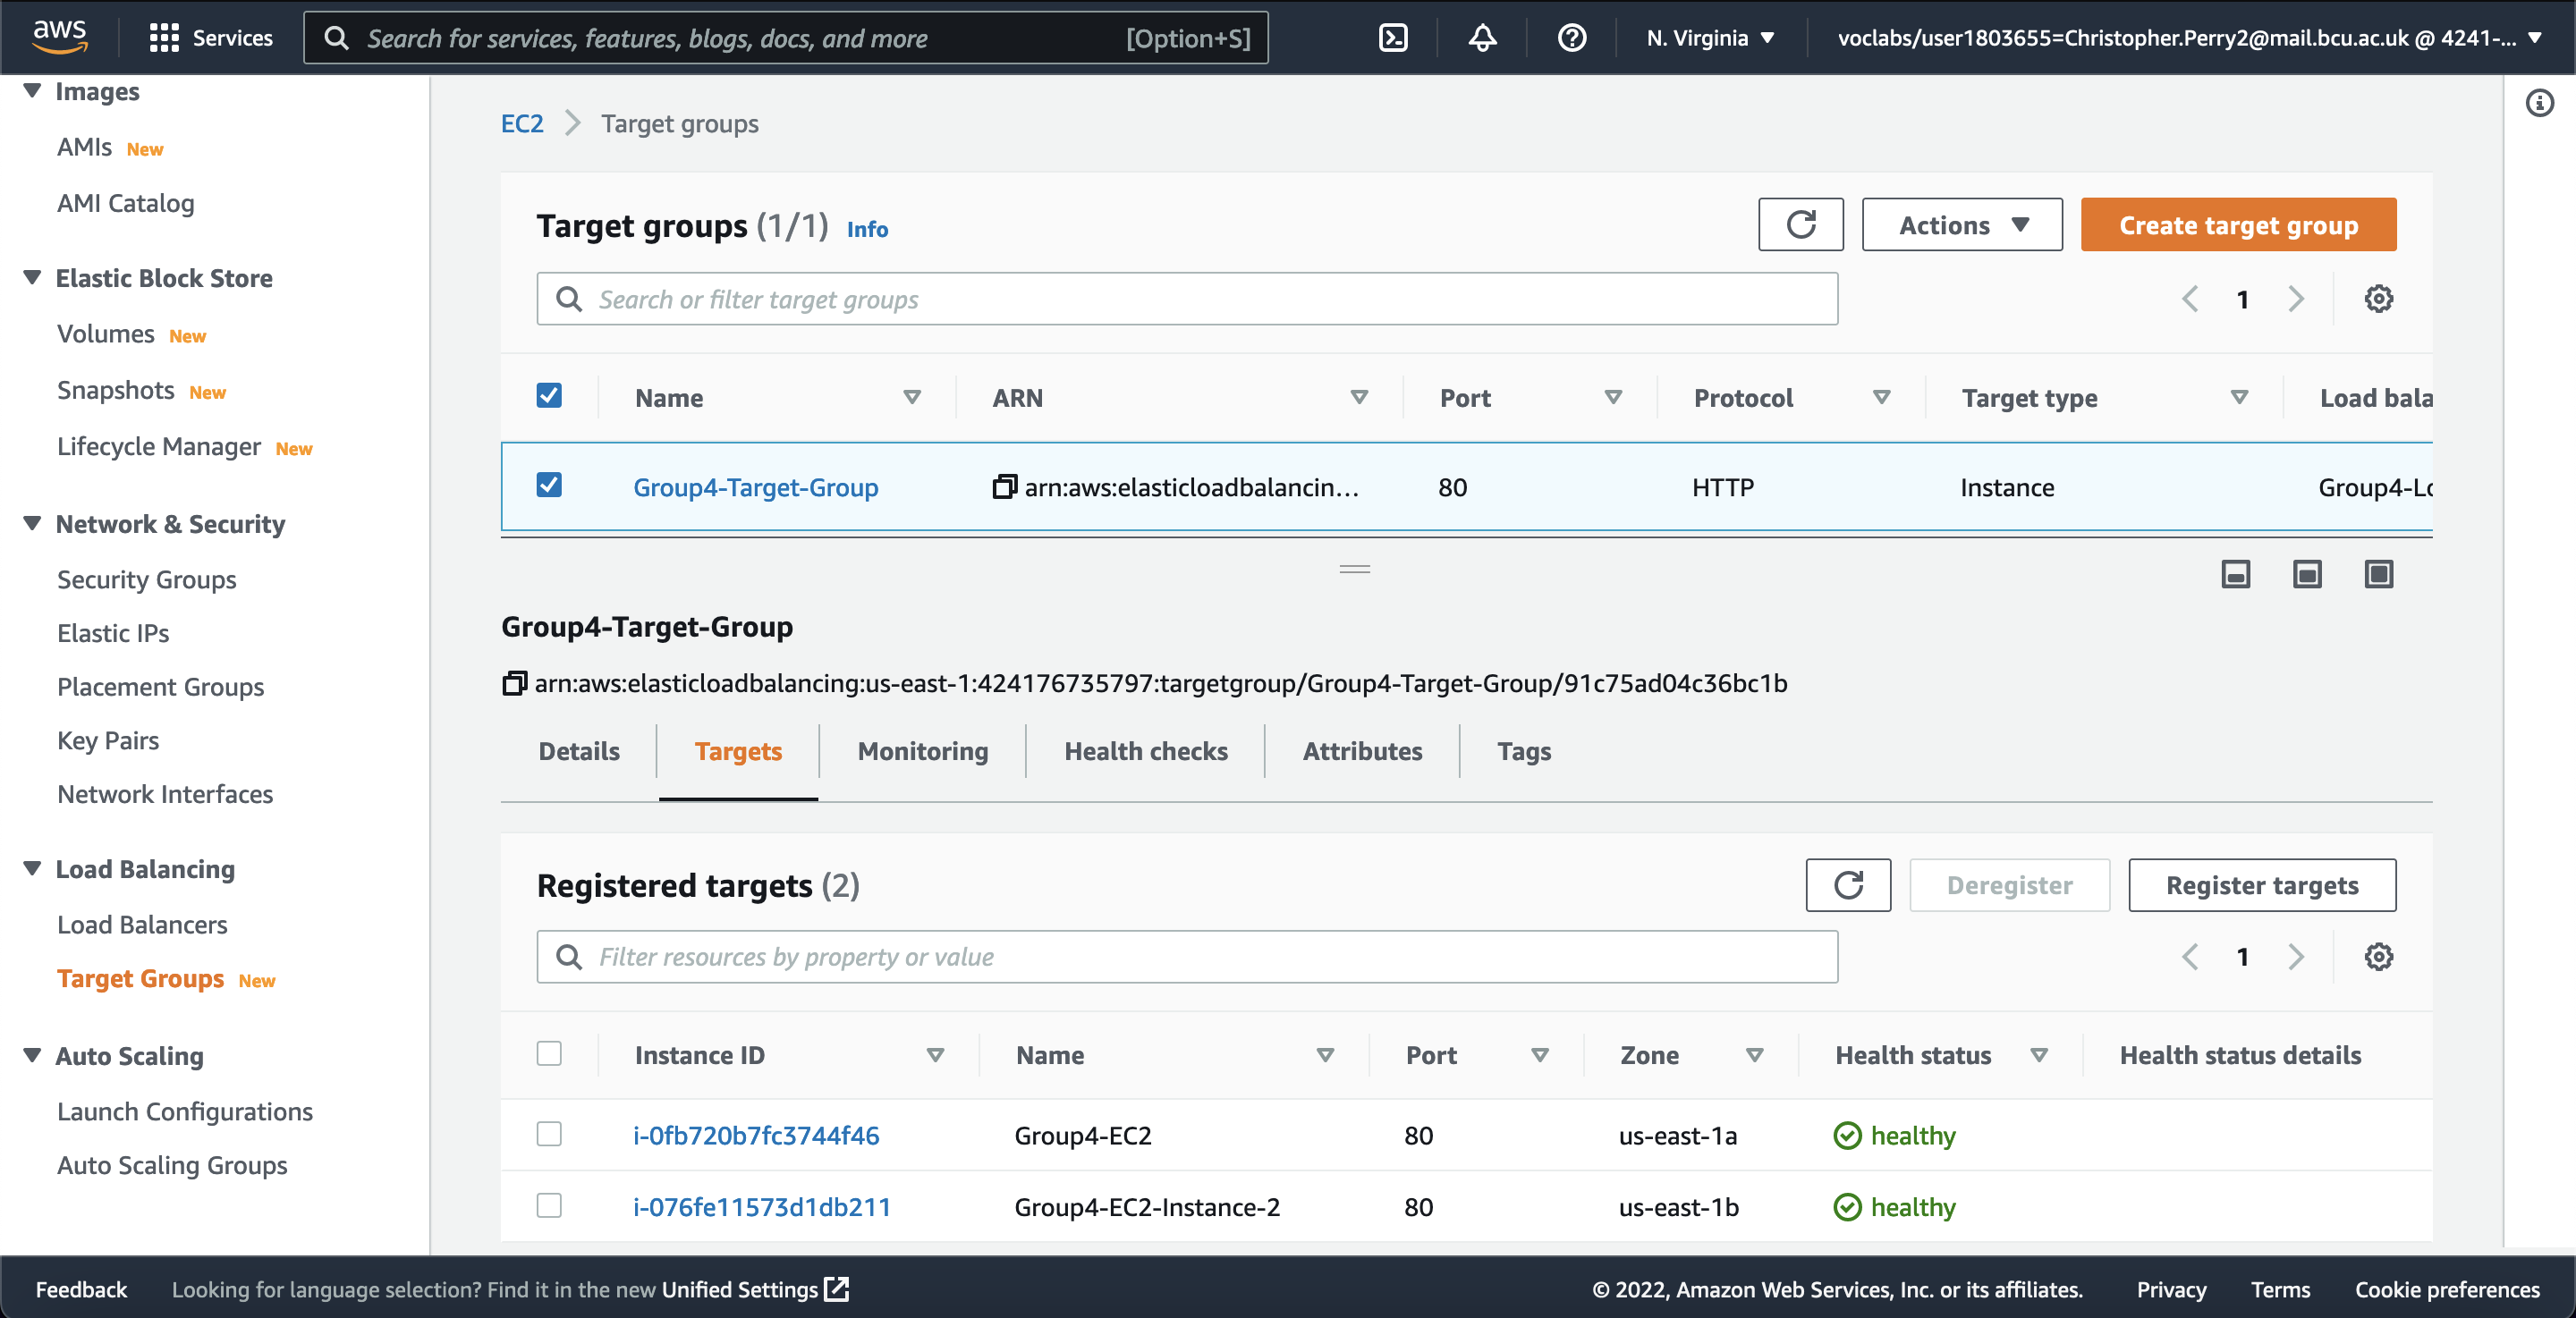
\includegraphics[width=\textwidth]{resources/elb/elb-target-group-created.png}
    \caption{Elastic Load Balancing}
    \label{fig:elb-target-group-create}
\end{figure}
\begin{figure}[!htbp]
    \centering
    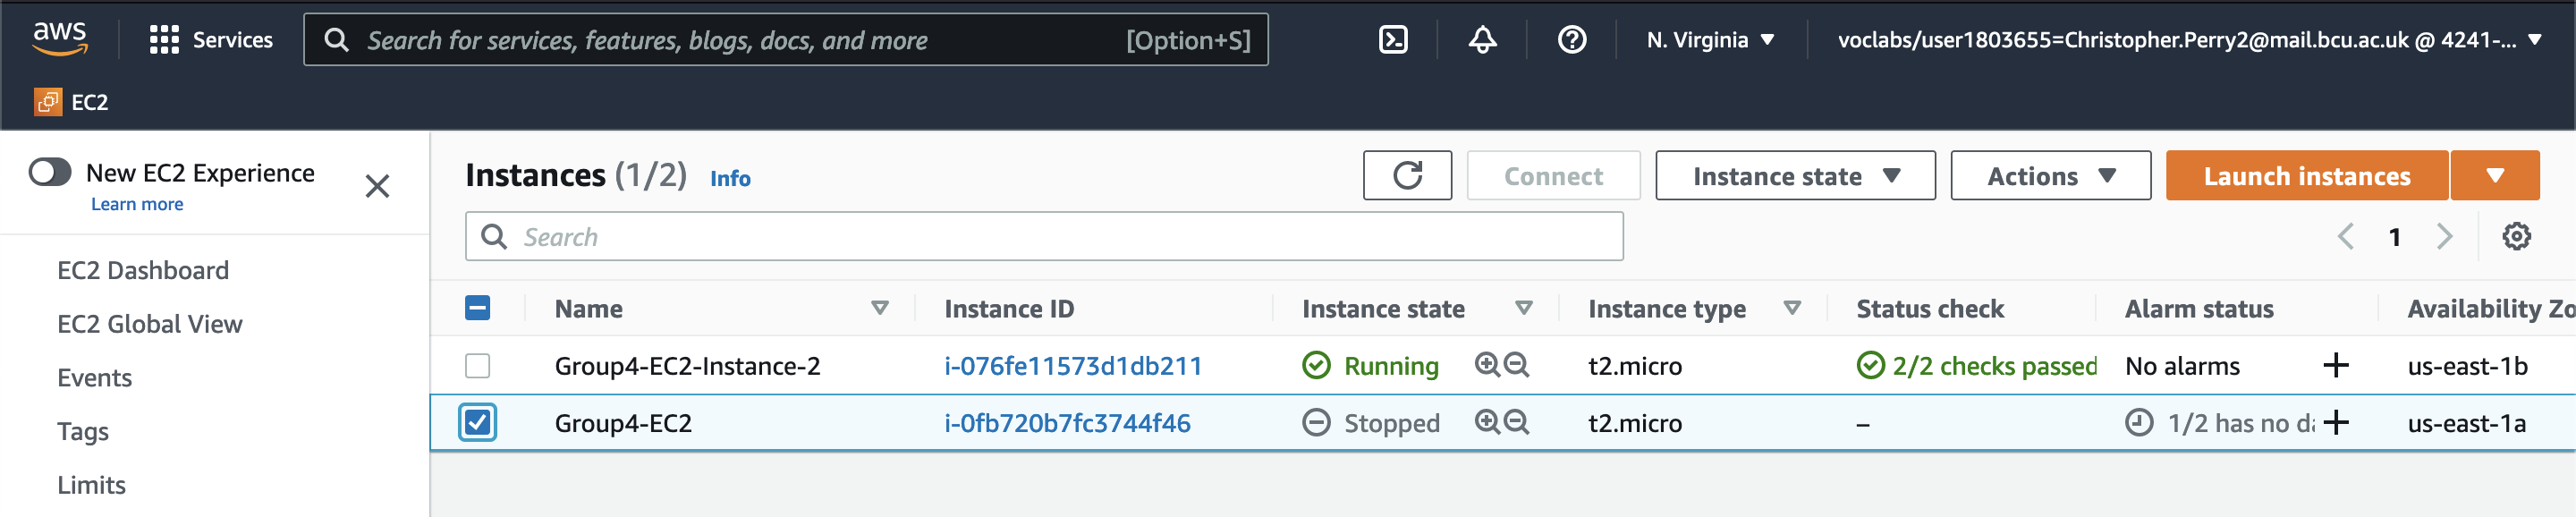
\includegraphics[width=\textwidth]{resources/elb/elb-test-stopped-instance.png}
    \caption{Elastic Load Balancing}
    \label{fig:elb-stopped-instance}
\end{figure}
\begin{figure}[!htbp]
    \centering
    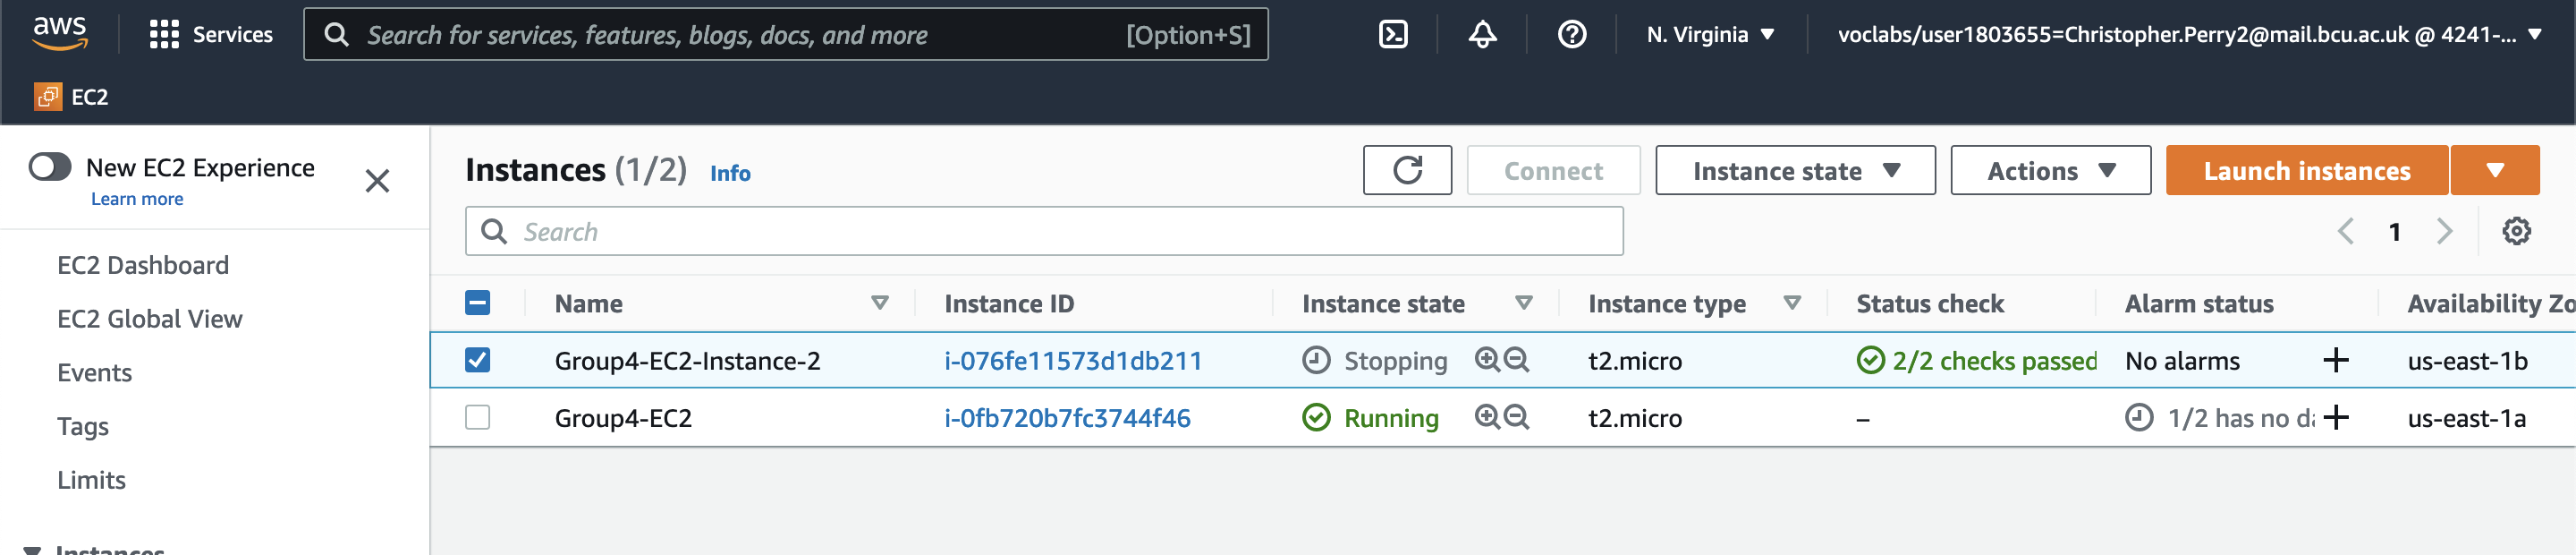
\includegraphics[width=\textwidth]{resources/elb/elb-test-stopped-instance-2.png}
    \caption{Elastic Load Balancing}
    \label{fig:elb-stopped-instance-2}
\end{figure}
\begin{figure}[!htbp]
    \centering
    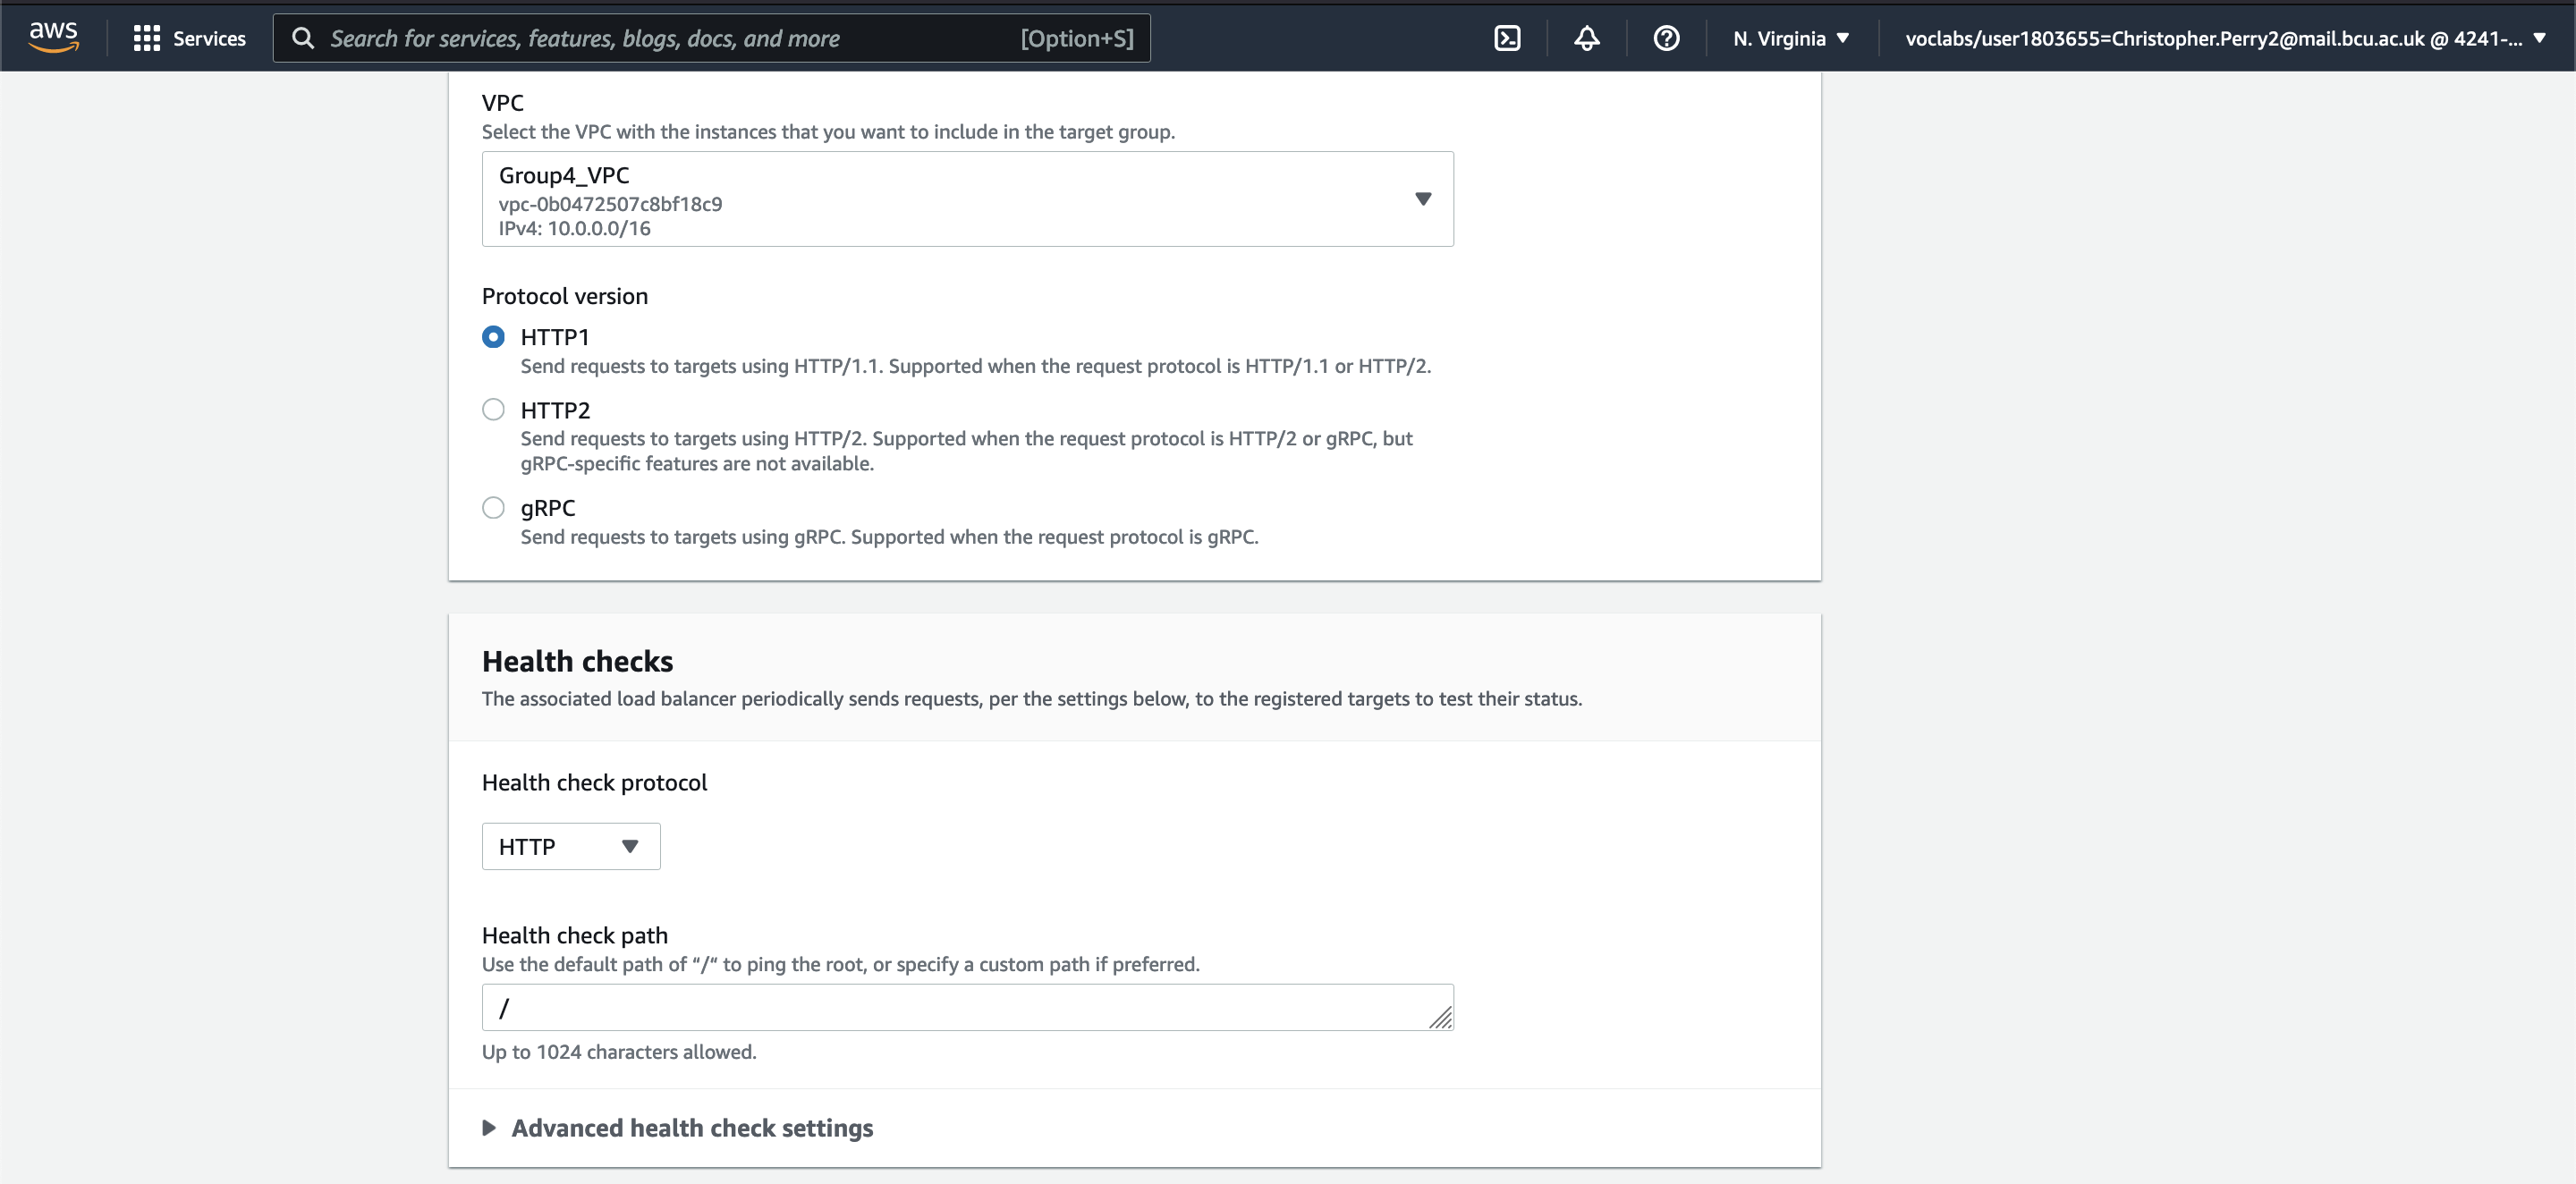
\includegraphics[width=\textwidth]{resources/elb/elb-vpc.png}
    \caption{Elastic Load Balancing}
    \label{fig:elb-vpc}
\end{figure}
\begin{figure}[!htbp]
    \centering
    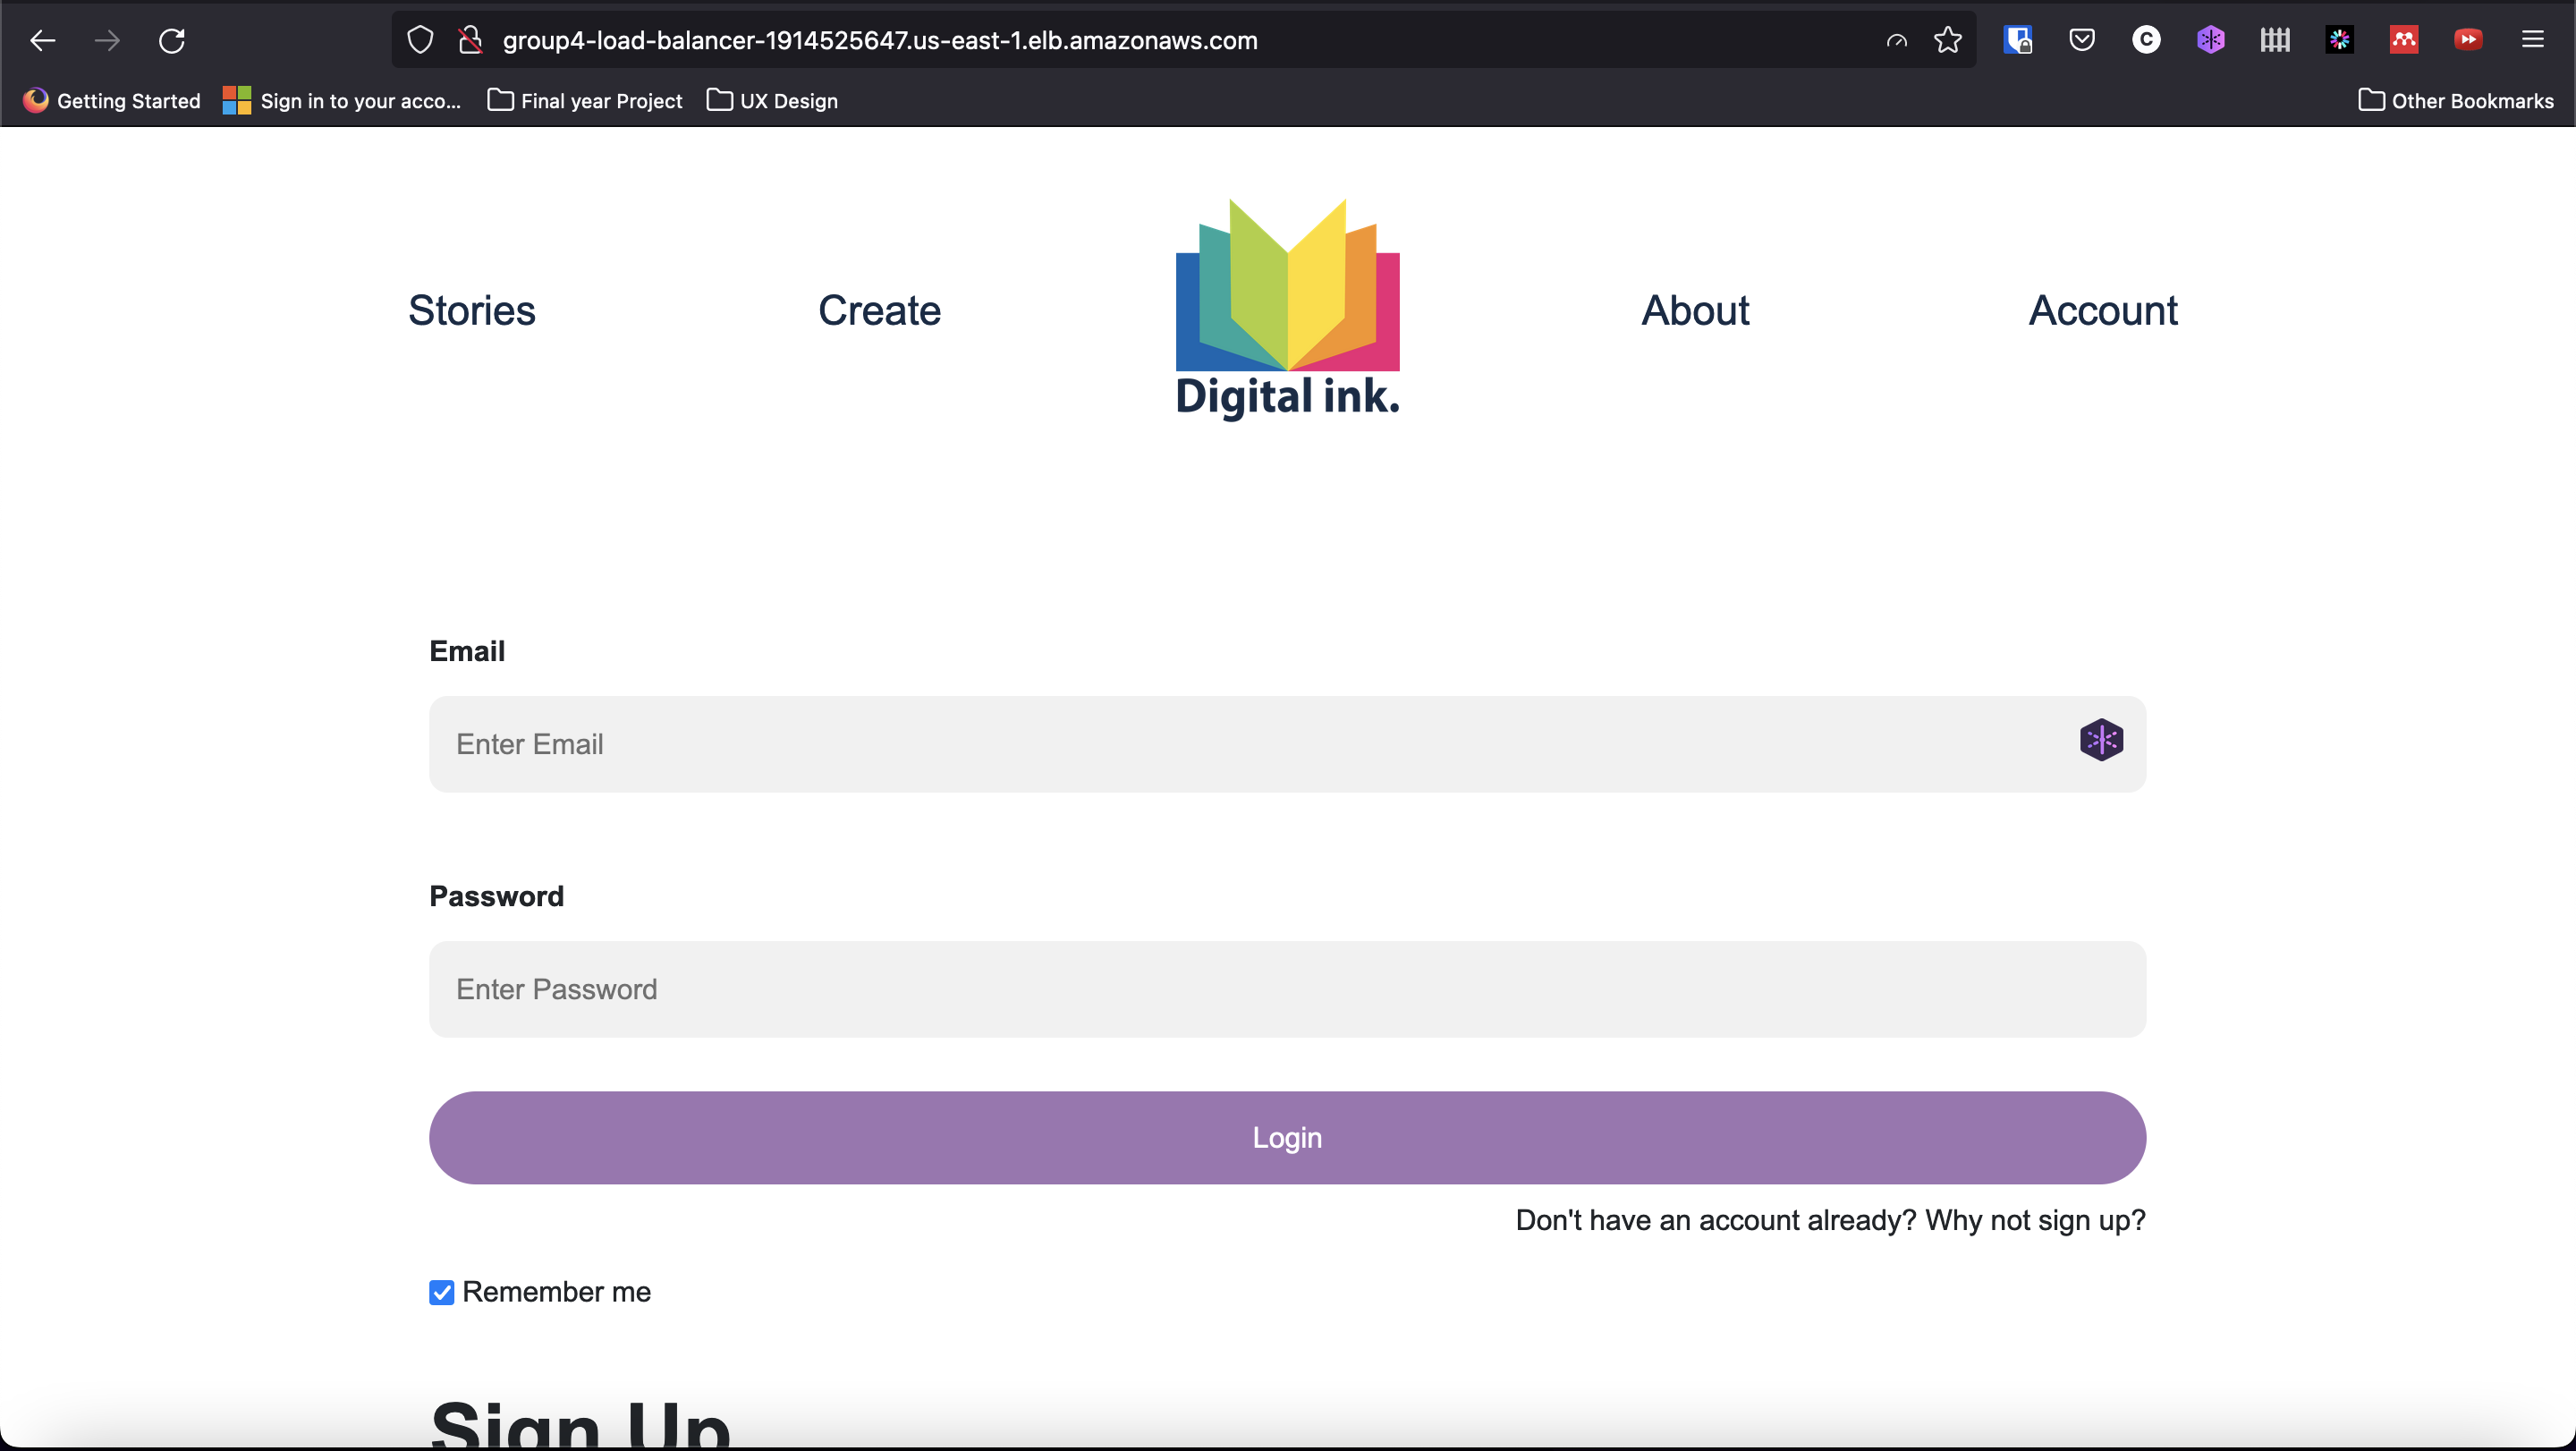
\includegraphics[width=\textwidth]{resources/elb/elb-working.png}
    \caption{Elastic Load Balancing}
    \label{fig:elb-working}
\end{figure}